% !TEX program = xelatex
\documentclass[11pt]{article}
\usepackage{fontspec}
\usepackage{xeCJK}
\usepackage[margin=1in]{geometry}
\usepackage{amsmath}
\usepackage{amssymb}
\usepackage{amsthm}
\usepackage{graphicx}
\usepackage{tikz-cd}
\usepackage{multicol}
\usepackage{titling}
\usepackage{setspace}
\usepackage{float}
\usepackage{subcaption}
\usepackage{algorithm}
\usepackage{algpseudocode}
\newtheorem{theorem}{Theorem}
\newtheorem{lemma}{Lemma}

% Bigger & bolder title
\pretitle{\begin{center}\LARGE\bfseries}
\posttitle{\par\end{center}\vskip 0.5em}
\predate{\begin{center}}
\postdate{\end{center}}
\setlength{\droptitle}{-6em}

% Paragraph style (old)
% \setlength{\parindent}{0pt}
% \setlength{\parskip}{0.4\baselineskip}
% Paragraph style (new)
% \setlength{\parindent}{2em}
% \setlength{\parskip}{0pt}
% \setstretch{0.96}


\begin{document}

\title{Notes on ML Models}
\author{}
\date{}
\maketitle
\clearpage
\part{Mathematical Foundations}
This part is not aiming to provide a general coverage of all the mathematical foundations, but rather to provide a quick reference for the mathematical concepts that are frequently used and worth noting.
\section{Maximum Likelihood Estimation}
The process of estimating model parameters $\boldsymbol{\theta}$ from data $\mathcal{D}$ is called \textbf{model fitting}, or training, and is at the heart of machine learning.
The key optimization problem is,
\[
\hat{\boldsymbol{\theta}} = \operatorname*{argmax}_{\boldsymbol{\theta}} \mathcal{L}(\boldsymbol{\theta})
\]
where $\mathcal{L}(\boldsymbol{\theta})$ is some kind of loss function or objective function.

The most common approach to parameter estimation is to pick the parameters that assign the highest
probability to the training data, called \textbf{maximum likelihood estimation} or \textbf{MLE}.
\[
\hat{\boldsymbol{\theta}}_{mle} = \operatorname*{argmax}_{\boldsymbol{\theta}} p(\mathcal{D} \mid \boldsymbol{\theta})
\]
Often, we assume the training examples are independently sampled from the same distribution (\textbf{iid} assumption),
\[
p(\mathcal{D} \mid \boldsymbol{\theta}) = \prod_{n=1}^N p(\mathbf{y}_n \mid \mathbf{x}_n, \boldsymbol{\theta})
\]
working with log likelihood 
\[
\hat{\boldsymbol{\theta}}_{mle} = \operatorname*{argmax}_{\boldsymbol{\theta}} \log p(\mathcal{D} \mid \boldsymbol{\theta}) = \operatorname*{argmax}_{\boldsymbol{\theta}} \sum_{n=1}^N \log p(\mathbf{y}_n \mid \mathbf{x}_n, \boldsymbol{\theta})
\]
In some tasks, the optimization algorithm is designed to minimize the loss function, so equivalently,
\[
\hat{\boldsymbol{\theta}}_{mle} = \operatorname*{argmin}_{\boldsymbol{\theta}} \text{NLL}(\boldsymbol{\theta}) = \operatorname*{argmin}_{\boldsymbol{\theta}} - \sum_{n=1}^N \log p(\mathbf{y}_n \mid \mathbf{x}_n, \boldsymbol{\theta})
\]
In the special case of unsupervised learning, we have $\mathbf{x}_n = \emptyset$, so the MLE changes $p(\mathbf{y}_n \mid \mathbf{x}_n, \boldsymbol{\theta}) = p(\mathbf{y}_n \mid \boldsymbol{\theta})$

\subsection*{Justification}
To justify the use of the MLE is that the resulting predictive distribution $p(\boldsymbol{y}|\hat{\boldsymbol{\theta}}_{\text{mle}})$ is as close as possible to the \textbf{empirical distribution} of the data. The empirical distribution is defined by
\[
p_{\mathcal{D}}(\boldsymbol{x}, \boldsymbol{y}) = p_{\mathcal{D}}(\boldsymbol{y}|\boldsymbol{x}) p_{\mathcal{D}}(\boldsymbol{x}) = \frac{1}{N} \sum_{n=1}^{N} \delta(\boldsymbol{x} - \boldsymbol{x}_n) \delta(\boldsymbol{y} - \boldsymbol{y}_n)
\]
the empirical distribution is a series of delta functions at the observed training points.

If we define $q(Y \mid \boldsymbol{x})$ denotes the model's predictive distribution, then the expected KL then becomes
\[
\begin{aligned}
\mathbb{E}_{p_{\mathcal{D}}(\boldsymbol{x})} \left[ D_{\mathbb{KL}} \left( p_{\mathcal{D}}(Y|\boldsymbol{x}) \, \| \, q(Y|\boldsymbol{x}) \right) \right] &= \sum_{\boldsymbol{x}} p_{\mathcal{D}}(\boldsymbol{x}) \left[ \sum_{\boldsymbol{y}} p_{\mathcal{D}}(\boldsymbol{y}|\boldsymbol{x}) \log \frac{p_{\mathcal{D}}(\boldsymbol{y}|\boldsymbol{x})}{q(\boldsymbol{y}|\boldsymbol{x})} \right] \\
&= \text{const} - \sum_{\boldsymbol{x}, \boldsymbol{y}} p_{\mathcal{D}}(\boldsymbol{x}, \boldsymbol{y}) \log q(\boldsymbol{y}|\boldsymbol{x}) \\
&= \text{const} - \frac{1}{N} \sum_{n=1}^{N} \log p(\boldsymbol{y}_n | \boldsymbol{x}_n, \boldsymbol{\theta})
\end{aligned}
\]
Minimizing the expected KL divergence is equivalent to minimizing the conditional NLL.

\section{Mixture Models}
To create more complex probability models is to take a convex combination of simple
distributions. This is called a mixture model.
\[
p(\boldsymbol{y}|\boldsymbol{\theta}) = \sum_{k=1}^{K} p(z=k|\boldsymbol{\theta}) p(\boldsymbol{y}|z=k, \boldsymbol{\theta}) = \sum_{k=1}^{K} \pi_k p(\boldsymbol{y}|z=k, \boldsymbol{\theta})
\]
$\pi_k$ is the mixture weight for component $k$, and $\sum_{k=1}^{K} \pi_k = 1$, and the \textbf{latent variable} $z \in \{1, \ldots, K\}$ which specifies which distribution to use for generating the output $\boldsymbol{y}$.

A \textbf{Gaussian mixture models (GMM)} is a mixture model where each component is a Gaussian distribution,
\[
p(\boldsymbol{y}|\boldsymbol{\theta}) = \sum_{k=1}^{K} \pi_k \mathcal{N}(\boldsymbol{y}|\boldsymbol{\mu}_k, \boldsymbol{\Sigma}_k)
\]

GMMs are often used for unsupervised clustering of real-valued data samples $\boldsymbol{y}_n \in \mathbb{R}^D$. 
First, the parameters $\boldsymbol{\theta}$ of the GMM can be estimated using MLE, often with the Expectation-Maximization (EM) algorithm.
\[
\hat{\boldsymbol{\theta}} = \operatorname*{argmax}_{\boldsymbol{\theta}} \log p(\{\boldsymbol{y}_n : n = 1, \ldots, N\} \mid \boldsymbol{\theta})
\]
Then, we associate each data point $\boldsymbol{y}_n$ with a discrete latent variable $z_n \in \{1, \ldots, K\}$, which indicates which mixture component or cluster generated the data point. The posterior distribution over the latent variable is given by Bayes' rule:
\[
p(z_n=k|\boldsymbol{y}_n, \boldsymbol{\theta}) = \frac{p(\boldsymbol{y}_n|z_n=k, \boldsymbol{\theta}) p(z_n=k|\boldsymbol{\theta})}{\sum_{j=1}^{K} p(\boldsymbol{y}_n|z_n=j, \boldsymbol{\theta}) p(z_n=j|\boldsymbol{\theta})} 
\]
This quantity is known as the \textbf{responsibility} of cluster $k$ for data point $\boldsymbol{y}_n$. Then, we can compute the most probable cluster assignment as:
\[
\hat{z}_n = \operatorname*{argmax}_{k} p(z_n=k|\boldsymbol{y}_n, \boldsymbol{\theta})
\]
This forms the basis of the clustering alorithms like the K-means clustering.

A \textbf{Bernoulli mixture model (BMM)} can be used for binary-valued data, where each mixture component has the following form:
\[
p(\boldsymbol{y}|z=k, \boldsymbol{\theta}) = \prod_{d=1}^{D} \text{Ber}(y_d | \mu_{dk}) = \prod_{d=1}^{D} \mu_{dk}^{y_d} (1 - \mu_{dk})^{1-y_d}
\]

\section{Matrix Calculus}
\subsection{Functions that map scalars to scalars}

A scalar-argument function $f : \mathbb{R} \to \mathbb{R}$, its derivative is defined as
\[
f'(x) = \lim_{h \to 0} \frac{f(x + h) - f(x)}{h}
\]
It can be interpreted as the slope of the tangent line at $f(x)$, and hence
\[
f(x + h) \approx f(x) + f'(x)h
\]

\subsection{Functions that map vectors to scalars}
A vector-argument functions, $f : \mathbb{R}^n \to \mathbb{R}$, by defining
the \textbf{partial derivative} of $f$ with respect to $x_i$ to be

\[
\frac{\partial f}{\partial x_i} = \lim_{h \to 0} \frac{f(\boldsymbol{x} + h\boldsymbol{e}_i) - f(\boldsymbol{x})}{h}
\]
where $\boldsymbol{e}_i$ is the $i$'th unit vector.

The \textbf{gradient} of a function at a point $\boldsymbol{x}$ is the vector of its partial derivatives:
\[
\boldsymbol{g} = \frac{\partial f}{\partial \boldsymbol{x}} = \nabla f = \begin{pmatrix} \frac{\partial f}{\partial x_1} \\ \vdots \\ \frac{\partial f}{\partial x_n} \end{pmatrix}
\]

The \textbf{directional derivative} measures how much the function $f : \mathbb{R}^n \to \mathbb{R}$ changes along a direction $\boldsymbol{v}$ in space,
\[
D_{\boldsymbol{v}} f(\boldsymbol{x}) = \lim_{h \to 0} \frac{f(\boldsymbol{x} + h\boldsymbol{v}) - f(\boldsymbol{x})}{h} = \nabla f^\top \boldsymbol{v}
\]

Suppose that some of the arguments to the function depend on each other $f(t, x(t), y(t))$. The \textbf{total derivative} of $f$ wrt $t$ is:
\[
\frac{df}{dt} = \frac{\partial f}{\partial t} + \frac{\partial f}{\partial x} \frac{dx}{dt} + \frac{\partial f}{\partial y} \frac{dy}{dt}
\]
then \textbf{total differential},
\[
df = \frac{\partial f}{\partial t} dt + \frac{\partial f}{\partial x} dx + \frac{\partial f}{\partial y} dy
\]
This measures how much $f$ changes when we change $t$, both via the direct effect of $t$ on $f$, but also indirectly, via the effects of $t$ on $x$ and $y$.

The \textbf{Hessian matrix} is the (symmetric) $n \times n$ matrix of second partial derivatives:
\[
\mathbf{H}_f = \frac{\partial^2 f}{\partial \boldsymbol{x}^2} = \nabla^2 f = \begin{pmatrix} \dfrac{\partial^2 f}{\partial x_1^2} & \cdots & \dfrac{\partial^2 f}{\partial x_1 \partial x_n} \\ & \vdots & \\ \dfrac{\partial^2 f}{\partial x_n \partial x_1} & \cdots & \dfrac{\partial^2 f}{\partial x_n^2} \end{pmatrix}
\]
the Hessian is the Jacobian of the gradient.

Consider a differentiable function $f: \mathbb{R}^n \to \mathbb{R}$. Here are some useful identities:
\[
\frac{\partial (\boldsymbol{a}^\mathsf{T} \boldsymbol{x})}{\partial \boldsymbol{x}} = \boldsymbol{a}
\]
\[
\frac{\partial (\boldsymbol{b}^\mathsf{T} \mathbf{A} \boldsymbol{x})}{\partial \boldsymbol{x}} = \mathbf{A}^\mathsf{T} \boldsymbol{b}
\]
\[
\frac{\partial (\boldsymbol{x}^\mathsf{T} \mathbf{A} \boldsymbol{x})}{\partial \boldsymbol{x}} = (\mathbf{A} + \mathbf{A}^\mathsf{T}) \boldsymbol{x}
\]

\subsection{Functions that map vectors to vectors}
A function that maps a vector to another vector, $f : \mathbb{R}^n \to \mathbb{R}^m$, can be written as
\[
f(\boldsymbol{x}) = \begin{pmatrix} f_1(\boldsymbol{x}) \\ \vdots \\ f_m(\boldsymbol{x}) \end{pmatrix}
\]
where each component $f_i : \mathbb{R}^n \to \mathbb{R}$ is a scalar-valued function. The \textbf{Jacobian matrix} of this function is an $m \times n$ matrix of partial derivatives:
\[
\mathbf{J}_{\boldsymbol{f}}(\boldsymbol{x}) = \frac{\partial \boldsymbol{f}}{\partial \boldsymbol{x}^\mathsf{T}} \triangleq \begin{pmatrix} \dfrac{\partial f_1}{\partial x_1} & \cdots & \dfrac{\partial f_1}{\partial x_n} \\ \vdots & \ddots & \vdots \\ \dfrac{\partial f_m}{\partial x_1} & \cdots & \dfrac{\partial f_m}{\partial x_n} \end{pmatrix} = \begin{pmatrix} \nabla f_1(\boldsymbol{x})^\mathsf{T} \\ \vdots \\ \nabla f_m(\boldsymbol{x})^\mathsf{T} \end{pmatrix}
\in \mathbb{R}^{m \times n}
\]

There are two ways to multiply the Jacobian with a vector:
\begin{itemize}
    \item Jacobian vector product (JVP): $\mathbf{J}_{\boldsymbol{f}}(\boldsymbol{x}) \boldsymbol{v} = \begin{pmatrix} \nabla f_1(\boldsymbol{x})^\mathsf{T} \\ \vdots \\ \nabla f_m(\boldsymbol{x})^\mathsf{T} \end{pmatrix} \boldsymbol{v} = \begin{pmatrix} \nabla f_1(\boldsymbol{x})^\mathsf{T} \boldsymbol{v} \\ \vdots \\ \nabla f_m(\boldsymbol{x})^\mathsf{T} \boldsymbol{v} \end{pmatrix}$.
    \item Vector Jacobian product (VJP): $\boldsymbol{u}^\mathsf{T} \mathbf{J}_{\boldsymbol{f}}(\boldsymbol{x}) = \boldsymbol{u}^\mathsf{T} \left( \frac{\partial \boldsymbol{f}}{\partial x_1}, \cdots, \frac{\partial \boldsymbol{f}}{\partial x_n} \right) = \left( \boldsymbol{u} \cdot \frac{\partial \boldsymbol{f}}{\partial x_1}, \cdots, \boldsymbol{u} \cdot \frac{\partial \boldsymbol{f}}{\partial x_n} \right)$.
\end{itemize}

Let $h(\boldsymbol{x}) = g(f(\boldsymbol{x}))$, by the chain rule of calculus,
\[
\mathbf{J}_h(\boldsymbol{x}) = \mathbf{J}_g(f(\boldsymbol{x})) \mathbf{J}_f(\boldsymbol{x})
\]

\subsection{Functions that map matrices to scalars}
A function $f: \mathbb{R}^{m \times n} \to \mathbb{R}$,
\[
\frac{\partial f}{\partial \mathbf{X}} = \begin{pmatrix} \dfrac{\partial f}{\partial x_{11}} & \cdots & \dfrac{\partial f}{\partial x_{1n}} \\ & \vdots & \\ \dfrac{\partial f}{\partial x_{m1}} & \cdots & \dfrac{\partial f}{\partial x_{mn}} \end{pmatrix}
\]
Here are some useful identities:
\[
\frac{\partial}{\partial \mathbf{X}} (\boldsymbol{a}^\mathsf{T} \mathbf{X} \boldsymbol{b}) = \boldsymbol{a} \boldsymbol{b}^\mathsf{T}
\]
\[
\frac{\partial}{\partial \mathbf{X}} (\boldsymbol{a}^\mathsf{T} \mathbf{X}^\mathsf{T} \boldsymbol{b}) = \boldsymbol{b} \boldsymbol{a}^\mathsf{T}
\]
\[
\frac{\partial}{\partial \mathbf{X}} \text{tr}(\mathbf{A} \mathbf{X} \mathbf{B}) = \mathbf{A}^\mathsf{T} \mathbf{B}^\mathsf{T}
\]
\[
\frac{\partial}{\partial \mathbf{X}} \text{tr}(\mathbf{X}^\mathsf{T} \mathbf{A}) = \mathbf{A}
\]
\[
\frac{\partial}{\partial \mathbf{X}} \text{tr}(\mathbf{X}^{-1} \mathbf{A}) = -\mathbf{X}^{-\mathsf{T}} \mathbf{A}^\mathsf{T} \mathbf{X}^{-\mathsf{T}}
\]
\[
\frac{\partial}{\partial \mathbf{X}} \text{tr}(\mathbf{X}^\mathsf{T} \mathbf{A} \mathbf{X}) = (\mathbf{A} + \mathbf{A}^\mathsf{T}) \mathbf{X}
\]
\[
\frac{\partial}{\partial \mathbf{X}} \det(\mathbf{A} \mathbf{X} \mathbf{B}) = \det(\mathbf{A} \mathbf{X} \mathbf{B}) \mathbf{X}^{-\mathsf{T}}
\]
\[
\frac{\partial}{\partial \mathbf{X}} \log(\det(\mathbf{X})) = \mathbf{X}^{-\mathsf{T}}
\]

\section{Bound Optimization}


\clearpage
\part{Linear Models and Neural Networks}
\section{Generalized Linear Models}

A GLM is a conditional version of an exponential family distribution $p(y \mid \theta) = h(y) \exp\left(\theta^\top T(y) - A(\theta)\right)$, in which the natural parameters are a linear function of the input. More precisely, the model has the following form:
\[
p(y_n \mid \mathbf{x}_n, \mathbf{w}, \sigma^2)
= \exp\left[\frac{y_n\eta_n - A(\eta_n)}{\sigma^2} + \log h(y_n, \sigma^2)\right]
\]
where 
\begin{itemize}
    \item $y_n$ is the output/response variable, $\mathbf{x_n}$ is the input/feature vector, $\mathbf{w}$ and $\sigma$ is the learnable model parameter 
    \item $\eta_n \triangleq \mathbf{w}^{\mathsf{T}}\mathbf{x}_n$ is the (input dependent) natural parameter or canonical parameter
    \item $A(\eta_n)$ is the log normalizer
    \item $\mathcal{T}(y_n) = y_n$ is the sufficient statistic, which is the smallest summary of the output data $y$ that retains everything relevant for estimating the parameter $\theta$ -- while it may still lose other information about $y$ itself.
    \item $\sigma^2$ is the dispersion term
    \item $h(y_n, \sigma^2)$  is the scaling constant or base measure
\end{itemize}

We can show that the mean and variance of the response variable are as follows:
\[
\int p(y_n \mid \eta_n, \sigma^2)\, dy_n = 1 \quad \text{for all } \eta_n
\]

To derive the mean, differentiate the equation w.r.t to $\eta_n$
\[ \int \frac{\partial p(y_n \mid \eta_n, \sigma^2)}{\partial \eta_n}\, dy_n = 0 \]
\[\int p(y_n\mid\eta_n,\sigma^2) \cdot \frac{y_n - A'(\eta_n)}{\sigma^2}\, dy_n = 0\]
\[\frac{1}{\sigma^2}\left[\int y_n\, p(y_n\mid\eta_n,\sigma^2)\, dy_n - A'(\eta_n)\right] = 0\]
thus, the \textbf{mean} is:
\[
\mathbb{E}\left[y_n \mid \mathbf{x}_n, \mathbf{w}, \sigma^2\right]
= A'(\eta_n) \triangleq \ell^{-1}(\eta_n)
\]
where the mapping from the linear inputs to the mean of the output using $\mu_n = \ell^{-1}(\eta_n)$, and the function $\ell$ is known as the link function, and $\ell^{-1}$ is known as the mean function. 

To derive the variance, differentiate the above equation w.r.t $\eta_n$ again,
\[
\int \left[-A''(\eta_n)\cdot p + (y_n - A'(\eta_n)) \cdot p \cdot \frac{y_n - A'(\eta_n)}{\sigma^2}\right] dy_n = 0
\]
\[-A''(\eta_n)\int p\, dy_n + \frac{1}{\sigma^2}\int (y_n - A'(\eta_n))^2\, p\, dy_n = 0
\]
thus, the \textbf{variance} is:
\[
\mathbb{V}\left[y_n \mid \mathbf{x}_n, \mathbf{w}, \sigma^2\right]
= A''(\eta_n)\sigma^2
\]

\subsection{Logistic regression}

Binary logistic regression is used when $y_n \in \{0,1\}$. It has the form
\[
p(y_n \mid \mathbf{x}_n, \mathbf{w})
= \mu_n^{y_n}(1-\mu_n)^{1-y_n}
\]
where
\[
\mu_n = \sigma(\eta_n) = \frac{1}{1 + \exp(-\eta_n)}, \quad
\eta_n = \mathbf{w}^{\mathsf{T}}\mathbf{x}_n.
\]
Hence
\[
\log p(y_n \mid \mathbf{x}_n, \mathbf{w})
= y_n\log \mu_n + (1-y_n)\log(1-\mu_n)
\]
Using $\mu_n = \exp(\eta_n)/(1+\exp(\eta_n))$, in GLM form:
\[
\log p(y_n \mid \mathbf{x}_n, \mathbf{w})
= y_n\eta_n - \log(1 + \exp(\eta_n))
\]
We see that $A(\eta_n) = \log(1 + \exp(\eta_n))$ and hence
\[
\mathbb{E}[y_n] = A'(\eta_n) = \frac{1}{1 + \exp(-\eta_n)},\quad \mathbb{V}[y_n] = A''(\eta_n) = \mu_n(1-\mu_n)
\]
Thus the link function is the logit function, $\ell(\mu_n) = \log\left(\frac{\mu_n}{1-\mu_n}\right)$, and the mean function is the sigmoid function, $\ell^{-1}(\eta_n) = \sigma(\eta_n)$.

\subsection{Linear regression}

Linear regression has the form with $y_n \in \mathbb{R}$
\[
p(y_n \mid \mathbf{x}_n, \mathbf{w}, \sigma^2)
= \frac{1}{\sqrt{2\pi\sigma^2}}
\exp\left(-\frac{1}{2\sigma^2}(y_n - \mathbf{w}^{\mathsf{T}}\mathbf{x}_n)^2\right)
\]
Hence
\[
\log p(y_n \mid \mathbf{x}_n, \mathbf{w}, \sigma^2)
= -\frac{1}{2\sigma^2}(y_n - \eta_n)^2 - \frac{1}{2}\log(2\pi\sigma^2)
\]
where $\eta_n = \mathbf{w}^{\mathsf{T}}\mathbf{x}_n$. In GLM form:
\[
\log p(y_n \mid \mathbf{x}_n, \mathbf{w}, \sigma^2)
= \frac{y_n\eta_n - \frac{\eta_n^2}{2}}{\sigma^2}
- \frac{1}{2}\left(\frac{y_n^2}{\sigma^2} + \log(2\pi\sigma^2)\right)
\]
We see that $A(\eta_n) = \eta_n^2/2$ and hence
\[
\mathbb{E}[y_n] = \eta_n = \mathbf{w}^{\mathsf{T}}\mathbf{x}_n,\quad \mathbb{V}[y_n] = \sigma^2 
\]

\subsection{Binomial regression}

If the response variable is the number of successes in $N_n$ trials, $y_n \in \{0,\ldots,N_n\}$, we can use binomial regression, which is defined by
\[
p(y_n \mid \mathbf{x}_n, N_n, \mathbf{w})
= \operatorname{Bin}(y_n \mid \sigma(\mathbf{w}^{\mathsf{T}}\mathbf{x}_n), N_n)
\]
note that binary logistic regression is the special case when $N_n = 1$. 

The log pdf is given by
\[
\log p(y_n \mid \mathbf{x}_n, N_n, \mathbf{w})
= y_n\log \mu_n + (N_n-y_n)\log(1-\mu_n) + \log \binom{N_n}{y_n}
\]
\[
= y_n\log\left(\frac{\mu_n}{1-\mu_n}\right)
+ N_n\log(1-\mu_n) + \log \binom{N_n}{y_n}
\]
where $\mu_n = \sigma(\eta_n)$. To rewrite this in GLM form, let us define
\[
\eta_n \triangleq \log\left(\frac{\mu_n}{1-\mu_n}\right)
= \log\left[\frac{1}{1+e^{-\mathbf{w}^{\mathsf{T}}\mathbf{x}_n}}\frac{1+e^{-\mathbf{w}^{\mathsf{T}}\mathbf{x}_n}}{e^{-\mathbf{w}^{\mathsf{T}}\mathbf{x}_n}}\right]
= \log\left(\frac{1}{e^{-\mathbf{w}^{\mathsf{T}}\mathbf{x}_n}}\right)
= \mathbf{w}^{\mathsf{T}}\mathbf{x}_n
\]
Hence we can write binomial regression in GLM form as follows:
\[
\log p(y_n \mid \mathbf{x}_n, N_n, \mathbf{w})
= y_n\eta_n - A(\eta_n) + h(y_n)
\]
where
\[
h(y_n) = \log \binom{N_n}{y_n}, \quad
A(\eta_n) = -N_n\log(1-\mu_n) = N_n\log(1+e^{\eta_n})
\]
Hence,
\[
\mathbb{E}[y_n] = \frac{dA}{d\eta_n} = \frac{N_n e^{\eta_n}}{1+e^{\eta_n}} = N_n \mu_n, \quad \mathbb{V}[y_n] = \frac{d^2A}{d\eta_n^2} = N_n \mu_n (1-\mu_n)
\]

\subsection{Poisson regression}

If the response variable is an integer count, $y_n \in \{0,1,\ldots\}$, we can use Poisson regression, which is defined by
\[
p(y_n \mid \mathbf{x}_n, \mathbf{w})
= \operatorname{Poi}(y_n \mid \exp(\mathbf{w}^{\mathsf{T}}\mathbf{x}_n))
\]
where
\[
\operatorname{Poi}(y \mid \mu) = e^{-\mu}\frac{\mu^y}{y!}
\]
is the Poisson distribution.

The log pdf is given by
\[
\log p(y_n \mid \mathbf{x}_n, \mathbf{w})
= y_n\log \mu_n - \mu_n - \log(y_n!)
\]
where $\mu_n = \exp(\mathbf{w}^{\mathsf{T}}\mathbf{x}_n)$. Hence in GLM form we have
\[
\log p(y_n \mid \mathbf{x}_n, \mathbf{w})
= y_n\eta_n - A(\eta_n) + h(y_n)
\]
where $\eta_n = \log(\mu_n) = \mathbf{w}^{\mathsf{T}}\mathbf{x}_n$, $A(\eta_n) = \mu_n = e^{\eta_n}$, and $h(y_n) = -\log(y_n!)$. Hence
\[
\mathbb{E}[y_n] = \frac{dA}{d\eta_n} = e^{\eta_n} = \mu_n, \quad
\mathbb{V}[y_n] = \frac{d^2A}{d\eta_n^2} = e^{\eta_n} = \mu_n
\]

\subsection{Canonical and non-canonical link functions}

Link functions connect three quantities:
\begin{itemize}
    \item $\theta_n$ --- the \textbf{natural parameter} of the \textit{exponential family distribution}.
    \item $\mu_n = \mathbb{E}[y_n]$ --- the \textbf{mean} of the output distribution.
    \item $\eta_n = \boldsymbol{w}^\top \boldsymbol{x}_n$ --- the \textbf{linear predictor}, built from the \textit{inputs} and weights.
\end{itemize}

\noindent The two connecting functions:
$$
\theta_n \xrightarrow{\ A'\ } \mu_n \xrightarrow{\ \ell\ } \eta_n
$$
\begin{itemize}
    \item $A'$ (derivative of the log-partition function) always maps $\theta_n \to \mu_n$. This relationship is fixed by the choice of exponential-family distribution (Bernoulli, Gaussian, Poisson, \ldots) and never changes.
    \item $\ell$, the \textbf{link function}, maps $\mu_n \to \eta_n$. This is the function \emph{you choose} when designing the GLM. Its inverse, $\ell^{-1}$, is the \textbf{mean function}: $\mu_n = \ell^{-1}(\eta_n)$ --- the direction actually used to generate predictions from $\eta_n$.
\end{itemize}

\textbf{Canonical link.} Choosing $\ell = (A')^{-1}$ makes the link exactly undo $A'$:
$$
\eta_n = g(\mu_n) = (A')^{-1}(A'(\theta_n)) = \theta_n
$$
so the natural parameter and linear predictor coincide: $\theta_n = \eta_n$.

\textbf{Non-canonical link.} Choosing any $g \ne (A')^{-1}$ gives
$$
\eta_n = g(A'(\theta_n)) \ne \theta_n \quad \text{in general.}
$$
The mean is still recovered correctly via $\mu_n = g^{-1}(\eta_n)$, but the natural parameter $\theta_n$ is no longer equal to the linear predictor $\eta_n$---recovering it requires the separate map $(A')^{-1}(\mu_n)$.

Examples of links:
\begin{itemize}
    \item Logit: canonical link $\theta_n = \ell(\mu_n) = \log\frac{\mu_n}{1-\mu_n}$.
    \item Complementary log-log: non-canonical link $\eta_n = \ell(\mu_n) = \log(-\log(1-\mu_n))$
\end{itemize}

\subsection{Maximum likelihood estimation}

GLMs can be fit the negative log-likelihood as the objective function (ignoring constant term $h$):
\[
\operatorname{NLL}(\mathbf{w})
= -\log p(\mathcal{D} \mid \mathbf{w})
= -\frac{1}{\sigma^2}\sum_{n=1}^{N}\ell_n 
= -\frac{1}{\sigma^2}\sum_{n=1}^{N}[\eta_n y_n - A(\eta_n)]
\]
where $\eta_n = \mathbf{w}^{\mathsf{T}}\mathbf{x}_n$. 

To find the MLE, we must solve $\nabla \text{NNL}(\mathbf{w}) = \mathbf{g(w)} = 0$. For notational simplicity, we will assume $\sigma^2 = 1$. The gradient for a single term is:
\[
\begin{aligned}
\mathbf{g}_n &= 
-\frac{1}{\sigma^2}\frac{\partial \ell_n}{\partial \mathbf{w}}
=-\frac{1}{\sigma^2} \frac{\partial \ell_n}{\partial \eta_n}\frac{\partial \eta_n}{\partial \mathbf{w}} \\
&=-\frac{1}{\sigma^2} \left(y_n - A'(\eta_n)\right)\mathbf{x}_n
=-\frac{1}{\sigma^2} (y_n - \mu_n)\mathbf{x}_n
\end{aligned}
\]
where $\mu_n = f(\mathbf{w^{\mathsf{T}} x})$, and $f$ is the inverse link function that maps from canonical parameters to mean parameters. If we interpret $(y_n - \mu_n)$ as an error signal, then the gradient $-\frac{1}{\sigma^2}\sum_{n=1}^{N}(y_n - \mu_n)\mathbf{x}_n$ weights each input $\mathbf{x}_n$ by its error, and averages the result.

Gradient-based optimization will find a stationary points where $\mathbf{g(w)} = 0$, we need to examine the Hessian matrix to determine whether it is the global optimum. The Hessian is given by 
\[
\begin{aligned}
\mathbf{H} &= \frac{\partial^2}{\partial \boldsymbol{w}\partial \boldsymbol{w}^\top}\text{NLL}(\boldsymbol{w}) \\ 
&= -\sum_{n=1}^N \frac{\partial \boldsymbol{g}_n}{\partial \boldsymbol{w}^\top}
= -\sum_{n=1}^N \frac{\partial \boldsymbol{g}_n}{\partial \mu_n}\frac{\partial \mu_n}{\partial \boldsymbol{w}^\top}
= -\sum_{n=1}^N \boldsymbol{x}_n f'(\boldsymbol{w}^\top \boldsymbol{x}_n)\boldsymbol{x}_n^\top
\end{aligned} 
\]
In general, the Hessian is positive definite, since $f'(\boldsymbol{w}^\top \boldsymbol{x}_n) > 0$, hence the negative log-likelihood is convex, so the MLE for a GLM is unique given $f(\boldsymbol{w}^\top \boldsymbol{x}_n) > 0$ for all $n$.

Based on these results, gradient-based optimizers can be used to estimate the model weights.

\subsubsection{Stochastic gradient descent}

The goal is to solve
\[
\hat{\boldsymbol{w}} \triangleq \operatorname*{argmin}_{\boldsymbol{w}} \mathcal{L}(\boldsymbol{w}) = \operatorname*{argmin}_{\boldsymbol{w}} \text{NLL}({\mathbf{w}})
\]
One of the methods is stochastic gradient descent: we use a minibatch from the whole dataset of size $N$, then we get the following update equation:
\[
\mathbf{w}_{t+1}
= \mathbf{w}_t - \alpha_t \nabla_{\mathbf{w}}\operatorname{NLL}(\mathbf{w}_t)
= \mathbf{w}_t - \alpha_t(\mu_n - y_n)\mathbf{x}_n
\]
where we replaced the average over all $N$ samples with a stochastically chosen minibatch size at each step $t$.

Since we know the objective is convex, then it can be shown that this will converge to a global optimum given the learning rate $\alpha_t$ is decayed appropriately at each step $t$.

\clearpage
\part{Dimentionality Reduction}
\section{Principal Component Analysis}
PCA algorithm is to find a \textbf{linear and orthogonal} projection of the high dimensional
data $x \in \mathbb{R}^D$, to a low dimensional subspace $z \in \mathbb{R}^L$, such that the low dimensional representation is a "good approximation" to the original data. If we project or encode $\mathbf{x}$ to get $\mathbf{z= W^T x}$, and then unproject or decode $\mathbf{z}$ to get $\mathbf{\hat{x}= Wz}$, then we want $\mathbf{x}$ to be close to $\mathbf{x}$ in $\ell_2$ distance. In particular, we can define the following \textbf{reconstruction error}:
\[
\mathcal{L}(\mathbf{W}) \triangleq \frac{1}{N}\sum_{n=1}^{N}
\left\lVert \mathbf{x}_n - \operatorname{decode}(\operatorname{encode}(\mathbf{x}_n;\mathbf{W});\mathbf{W}) \right\rVert_2^2
\]

PCA algorithm states that this objective can be minimized by setting $\mathbf{W} = \mathbf{U}_L$, where $\mathbf{U}_L$ contains the the $L$ eigenvectors with lages eigenvalues of the empirical covariance matrix 
\[
\hat{\boldsymbol{\Sigma}} = \frac{1}{N} \sum_{n=1}^N (\boldsymbol{x}_n - \overline{\boldsymbol{x}})(\boldsymbol{x}_n - \overline{\boldsymbol{x}})^\mathsf{T} = \frac{1}{N} \mathbf{X}_c^\mathsf{T}\mathbf{X}_c
\]
where $\mathbf{X}_c$ is a centered version of the $N \times D$ design matrix.

\subsection{PCA setup}
Suppose we have an (unlabeled) dataset $\mathcal{D} = \{\boldsymbol{x}_n : n = 1:N\}$, where $\boldsymbol{x}_n \in \mathbb{R}^D$. We can represent this as an $N \times D$ data matrix $\mathbf{X}$. We will assume $\overline{\boldsymbol{x}} = \frac{1}{N}\sum_{n=1}^N \boldsymbol{x}_n = \mathbf{0}$, which we can ensure by centering the data.

We would like to approximate each $\boldsymbol{x}_n$ by a low dimensional representation, $\boldsymbol{z}_n \in \mathbb{R}^L$. We assume that each $\boldsymbol{x}_n$ can be explained in terms of a weighted combination of basis functions $\boldsymbol{w}_1, \dots, \boldsymbol{w}_L$, where each $\boldsymbol{w}_k \in \mathbb{R}^D$, and where the weights are given by $\boldsymbol{z}_n \in \mathbb{R}^L$, i.e.
\[
\boldsymbol{x}_n \approx \sum_{k=1}^L z_{nk} \boldsymbol{w}_k
\]
The vector $\boldsymbol{z}_n$ is the low dimensional representation of $\boldsymbol{x}_n$, and is known as the \textbf{latent vector}, the collection of these latent variables are called the \textbf{latent factors}.

The error produced by this approximation:

\[
\mathcal{L}(\mathbf{W}, \mathbf{Z}) = \frac{1}{N} \|\mathbf{X} - \mathbf{Z}\mathbf{W}^\mathsf{T}\|_F^2 = \frac{1}{N} \|\mathbf{X}^\mathsf{T} - \mathbf{W}\mathbf{Z}^\mathsf{T}\|_F^2 = \frac{1}{N} \sum_{n=1}^N \|\boldsymbol{x}_n - \mathbf{W}\boldsymbol{z}_n\|^2
\]
where
\begin{itemize}
    \item $\mathbf{X} \in \mathbb{R}^{N \times D}$: data matrix, rows are centered data points $\mathbf{x}_n^T$
    \item $\mathbf{Z} \in \mathbb{R}^{N \times L}$: latent code matrix, rows are centered data points $\mathbf{z}_n^T$
    \item $\mathbf{W} \in \mathbb{R}^{D \times L}$: basis matrix, columns $\boldsymbol{w}_1, \dots, \boldsymbol{w}_L$ are orthonormal
    \item approximating each $\boldsymbol{x}_n$ by $\hat{\boldsymbol{x}}_n = \mathbf{W}\boldsymbol{z}_n$; or, $\hat{\mathbf{X}
    } = \mathbf{Z} \mathbf{W}^T$.
    \item the minimization of $\mathcal{L}$ is subject to constraints $\mathbf{w}_k^T \mathbf{w_j} = 0 \, \text{for}\, k \neq j \text{;}\, 1 \, \text{for}\, k = j$, i.e., $\mathbf{W}$ is orthogonal
\end{itemize}

\subsection{Algorithm derivation}
\textit{Base case}

Starting by considering the best 1d solution , $\mathbf{w}_1 \in \mathbb{R}^D$, letting the coefficients for each datapoints associated with the first basis vector be denoted by $\tilde{\mathbf{z}}_1 = [z_{11}, \dots , z_{N1}] \in \mathbb{R}^N$. The reconstruction error is 
\[
\begin{aligned}
\mathcal{L}(\boldsymbol{w}_1, \tilde{\boldsymbol{z}}_1) &= \frac{1}{N} \sum_{n=1}^N \|\boldsymbol{x}_n - z_{n1}\boldsymbol{w}_1\|^2 = \frac{1}{N} \sum_{n=1}^N (\boldsymbol{x}_n - z_{n1}\boldsymbol{w}_1)^\mathsf{T}(\boldsymbol{x}_n - z_{n1}\boldsymbol{w}_1) \\
&= \frac{1}{N} \sum_{n=1}^N [\boldsymbol{x}_n^\mathsf{T}\boldsymbol{x}_n - 2z_{n1}\boldsymbol{w}_1^\mathsf{T}\boldsymbol{x}_n + z_{n1}^2 \boldsymbol{w}_1^\mathsf{T}\boldsymbol{w}_1] \\ 
&= \frac{1}{N} \sum_{n=1}^N [\boldsymbol{x}_n^\mathsf{T}\boldsymbol{x}_n - 2z_{n1}\boldsymbol{w}_1^\mathsf{T}\boldsymbol{x}_n + z_{n1}^2]
\quad \text{since} \, \boldsymbol{w}_1^\mathsf{T}\boldsymbol{w}_1 = 1
\end{aligned}
\]

Taking derivatives wrt $z_{n1}$ and equating to zero gives
\[
\frac{\partial}{\partial z_{n1}} \mathcal{L}(\boldsymbol{w}_1, \tilde{\boldsymbol{z}}_1) = \frac{1}{N}[-2\boldsymbol{w}_1^\mathsf{T}\boldsymbol{x}_n + 2z_{n1}] = 0 \Rightarrow z_{n1} = \boldsymbol{w}_1^\mathsf{T}\boldsymbol{x}_n
\]
So the optimal embedding is obtained by orthogonally projecting the data onto $\boldsymbol{w}_1$. Plugging this back in gives the loss for the weights:

\[
\mathcal{L}(\boldsymbol{w}_1) = \mathcal{L}(\boldsymbol{w}_1, \tilde{\boldsymbol{z}}_1^*(\boldsymbol{w}_1)) = \frac{1}{N} \sum_{n=1}^N [\boldsymbol{x}_n^\mathsf{T}\boldsymbol{x}_n - z_{n1}^2] = \text{const} - \frac{1}{N} \sum_{n=1}^N z_{n1}^2
\]
To solve for $\boldsymbol{w}_1$, note that

\[
\mathcal{L}(\boldsymbol{w}_1) = -\frac{1}{N} \sum_{n=1}^N z_{n1}^2 = -\frac{1}{N} \sum_{n=1}^N \boldsymbol{w}_1^\mathsf{T}\boldsymbol{x}_n\boldsymbol{x}_n^\mathsf{T}\boldsymbol{w}_1 = -\boldsymbol{w}_1^\mathsf{T}\hat{\boldsymbol{\Sigma}}\boldsymbol{w}_1
\]
where $\boldsymbol{\Sigma}$ is the empirical covariance matrix (since we assumed the data is centered). We can trivially optimize this by letting $\|\boldsymbol{w}_1\| \to \infty$, so we impose the constraint $\|\boldsymbol{w}_1\| = 1$ and instead optimize

\[
\tilde{\mathcal{L}}(\boldsymbol{w}_1) = \boldsymbol{w}_1^\mathsf{T}\hat{\boldsymbol{\Sigma}}\boldsymbol{w}_1 - \lambda_1(\boldsymbol{w}_1^\mathsf{T}\boldsymbol{w}_1 - 1)
\]
where $\lambda_1$ is a Lagrange multiplier. Taking derivatives and equating to zero we have

\[
\frac{\partial}{\partial \boldsymbol{w}_1} \tilde{\mathcal{L}}(\boldsymbol{w}_1) = 2\hat{\boldsymbol{\Sigma}}\boldsymbol{w}_1 - 2\lambda_1 \boldsymbol{w}_1 = 0
\]

\[
\hat{\boldsymbol{\Sigma}}\boldsymbol{w}_1 = \lambda_1 \boldsymbol{w}_1
\]

Hence the optimal direction onto which we should project the data is an eigenvector of the covariance matrix. Left multiplying by $\boldsymbol{w}_1^\mathsf{T}$ (and using $\boldsymbol{w}_1^\mathsf{T}\boldsymbol{w}_1 = 1$) we find

\[
\boldsymbol{w}_1^\mathsf{T}\hat{\boldsymbol{\Sigma}}\boldsymbol{w}_1 = \lambda_1
\]
Since we want to maximize this quantity (minimize the loss), we pick the eigenvector which corresponds to the largest eigenvalue.

\par\medskip
\noindent \textit{Induction Step}

For another direction $\mathbf{w}_2$, the reconstructon error is
\[
\mathcal{L}(\boldsymbol{w}_1, \tilde{\boldsymbol{z}}_1, \boldsymbol{w}_2, \tilde{\boldsymbol{z}}_2) = \frac{1}{N} \sum_{n=1}^N \|\boldsymbol{x}_n - z_{n1}\boldsymbol{w}_1 - z_{n2}\boldsymbol{w}_2\|^2
\]
Optimizing wrt $\boldsymbol{w}_1$ and $\boldsymbol{z}_1$ gives the same solution as before. $\frac{\partial \mathcal{L}}{\partial \boldsymbol{z}_2} = 0$ yields $z_{n2} = \boldsymbol{w}_2^\mathsf{T}\boldsymbol{x}_n$. Substituting in yields
\[
\mathcal{L}(\boldsymbol{w}_2) = \frac{1}{N} \sum_{n=1}^N [\boldsymbol{x}_n^\mathsf{T}\boldsymbol{x}_n - \boldsymbol{w}_1^\mathsf{T}\boldsymbol{x}_n\boldsymbol{x}_n^\mathsf{T}\boldsymbol{w}_1 - \boldsymbol{w}_2^\mathsf{T}\boldsymbol{x}_n\boldsymbol{x}_n^\mathsf{T}\boldsymbol{w}_2] = \text{const} - \boldsymbol{w}_2^\mathsf{T}\hat{\boldsymbol{\Sigma}}\boldsymbol{w}_2
\]
Dropping the constant term, plugging in the optimal $\boldsymbol{w}_1$ and adding the constraints yields
\[
\tilde{\mathcal{L}}(\boldsymbol{w}_2) = -\boldsymbol{w}_2^\mathsf{T}\hat{\boldsymbol{\Sigma}}\boldsymbol{w}_2 + \lambda_2(\boldsymbol{w}_2^\mathsf{T}\boldsymbol{w}_2 - 1) + \lambda_{12}(\boldsymbol{w}_2^\mathsf{T}\boldsymbol{w}_1 - 0)
\]
with the extra constraint term, it can be shown that the solution is given by the eigenvector with the second largest eigenvalue:
\[
\hat{\boldsymbol{\Sigma}}\boldsymbol{w}_2 = \lambda_2 \boldsymbol{w}_2
\]
The proof continues in this way to show that $\hat{\mathbf{W}} = \mathbf{U}_L$.

\subsection{Computational tricks}
\begin{enumerate}
    \item \textbf{High-dimensional data.} PCA finds the eigenvectors of the $D \times D$ covariance matrix $\mathbf{X}^\mathsf{T}\mathbf{X}$. If $D > N$, it is faster to work with the $N \times N$ matrix $\mathbf{X}\mathbf{X}^\mathsf{T}$. Let $\mathbf{U}$ be an orthonormal matrix containing the eigenvectors of $\mathbf{X}\mathbf{X}^\mathsf{T}$ with corresponding eigenvalues in $\boldsymbol{\Lambda}$. By definition we have $(\mathbf{X}\mathbf{X}^\mathsf{T})\mathbf{U} = \mathbf{U}\boldsymbol{\Lambda}$. Pre-multiplying by $\mathbf{X}^\mathsf{T}$ gives
    \[
    (\mathbf{X}^\mathsf{T}\mathbf{X})(\mathbf{X}^\mathsf{T}\mathbf{U}) = (\mathbf{X}^\mathsf{T}\mathbf{U})\boldsymbol{\Lambda}
    \]
    from which we see that the eigenvectors of $\mathbf{X}^\mathsf{T}\mathbf{X}$ are $\mathbf{V} = \mathbf{X}^\mathsf{T}\mathbf{U}$, with eigenvalues $\boldsymbol{\Lambda}$ as before. However, these eigenvectors are not normalized, since $\|\boldsymbol{v}_j\|^2 = \boldsymbol{u}_j^\mathsf{T}\mathbf{X}\mathbf{X}^\mathsf{T}\boldsymbol{u}_j = \lambda_j \boldsymbol{u}_j^\mathsf{T}\boldsymbol{u}_j = \lambda_j$. The normalized eigenvectors are given by
    \[
    \mathbf{V} = \mathbf{X}^\mathsf{T}\mathbf{U}\boldsymbol{\Lambda}^{-\frac{1}{2}}
    \]
    \item \textbf{Computing PCA using SVD.} Let $\mathbf{U}_\Sigma \boldsymbol{\Lambda}_\Sigma \mathbf{U}_\Sigma^\mathsf{T}$ be the top $L$ eigendecomposition of the covariance matrix $\boldsymbol{\Sigma} \propto \mathbf{X}^\mathsf{T}\mathbf{X}$ (assume $\mathbf{X}$ is centered). Recall the optimal estimate of the projection weights $\mathbf{W}$ is given by the top $L$ eigenvalues, so $\mathbf{W} = \mathbf{U}_\Sigma$. Now let $\mathbf{U}_X \mathbf{S}_X \mathbf{V}_X^\mathsf{T} \approx \mathbf{X}$ be the $L$-truncated SVD approximation to the data matrix $\mathbf{X}$. By SVD definition, the columns of $\mathbf{V}_X$ are the eigenvectors of $\mathbf{X}^\mathsf{T}\mathbf{X}$, so 
    \[
    \mathbf{V}_X = \mathbf{U}_\Sigma = \mathbf{W}.
    \]
    In addition, the eigenvalues of the covariance matrix are related to the singular values of the data matrix via $\lambda_k = s_k^2/N$. Now suppose we are interested in the principal components (or PC scores), rather than the projection matrix. We have
    \[
    \mathbf{Z} = \mathbf{X}\mathbf{W} = \mathbf{U}_X \mathbf{S}_X \mathbf{V}_X^\mathsf{T} \mathbf{V}_X = \mathbf{U}_X \mathbf{S}_X
    \]
    Finally, if we want to approximately reconstruct the data, we have
    \[
    \hat{\mathbf{X}} = \mathbf{Z}\mathbf{W}^\mathsf{T} = \mathbf{U}_X \mathbf{S}_X \mathbf{V}_X^\mathsf{T}
    \]
    This is precisely the same as a \textbf{truncated SVD approximation}.
    \item \textbf{Latent dimentions selection}. Recall that the reconstruction error can be written in terms of eigenvalues 
    \[
    \mathcal{L}_L = \frac{1}{|\mathcal{D}|} \sum_{n \in \mathcal{D}} \|\boldsymbol{x}_n - \hat{\boldsymbol{x}}_n\|^2 = \sum_{j=L+1}^{D}\lambda_j
    \]
    where $\hat{\mathbf{x}}_n = \mathbf{Wz}_n + \mathbf{\mu}$ and $\mathbf{\mu}$ is the empirical mean. Thus, as the number of dimentions incrceases, the eigenvalues get smaller, and so does the reconstruction error. Therefore, if we give it more latent dimenions, it will be able to approximate the test date more accurately.
\end{enumerate}
Thus, PCA can be performed either using an eigendecomposition of $\boldsymbol{\Sigma}$ or an SVD decomposition of $\mathbf{X}$. The latter is often preferable, for computational reasons.

\clearpage
\section{Factor Analysis}
Factor analysis is a generalization of PCA corresponds to the following linear-Gaussian latent variable probabilistic \textbf{generative} model:
\[ 
\mathbf{x} = \mathbf{W}\mathbf{z} + \boldsymbol{\mu} + \boldsymbol{\epsilon}, \quad \boldsymbol{\epsilon} \sim \mathcal{N}(\mathbf{0}, \boldsymbol{\Psi})   
\]
\[
p(\boldsymbol{z}) = \mathcal{N}(\boldsymbol{z} \mid \boldsymbol{\mu}_0, \boldsymbol{\Sigma}_0)
\]
\[
p(\boldsymbol{x} \mid \boldsymbol{z}, \boldsymbol{\theta}) = \mathcal{N}(\boldsymbol{x} \mid \mathbf{W}\boldsymbol{z} + \boldsymbol{\mu}, \boldsymbol{\Psi})
\]
where $\mathbf{W}$ is a $D \times L$ matrix, known as the \textbf{factor loading matrix}, $\boldsymbol{\Psi}$ is a diagonal $D \times D$ noise covariance matrix, and $\boldsymbol{\mu}$ is a $D \times 1$ mean of observed data

FA can be thought of as a low-rank version of a Gaussian distribution. To see this, note that the induced marginal distribution $p(\boldsymbol{x} \mid \boldsymbol{\theta})$ is a Gaussian:
\[
p(\boldsymbol{x} \mid \boldsymbol{\theta}) = \int \mathcal{N}(\boldsymbol{x} \mid \mathbf{W}\boldsymbol{z} + \boldsymbol{\mu}, \boldsymbol{\Psi}) \mathcal{N}(\boldsymbol{z} \mid \boldsymbol{\mu}_0, \boldsymbol{\Sigma}_0) \, d\boldsymbol{z}
\]
\[
= \mathcal{N}(\boldsymbol{x} \mid \mathbf{W}\boldsymbol{\mu}_0 + \boldsymbol{\mu}, \boldsymbol{\Psi} + \mathbf{W}\boldsymbol{\Sigma}_0\mathbf{W}^\mathsf{T})
\]
Hence $\mathbb{E}[\boldsymbol{x}] = \mathbf{W}\boldsymbol{\mu}_0 + \boldsymbol{\mu}$ and $\text{Cov}[\boldsymbol{x}] = \mathbf{W}\text{Cov}[\boldsymbol{z}]\mathbf{W}^\mathsf{T} + \boldsymbol{\Psi} = \mathbf{W}\boldsymbol{\Sigma}_0\mathbf{W}^\mathsf{T} + \boldsymbol{\Psi}$. Without loss of generality, we can set $\boldsymbol{\mu}_0 = \mathbf{0}$ and $\boldsymbol{\Sigma}_0 = \boldsymbol{I}$. Thus,
\[
p(\boldsymbol{z}) = \mathcal{N}(\boldsymbol{z} \mid \mathbf{0}, \mathbf{I})
\]
\[
p(\boldsymbol{x} \mid \boldsymbol{z}) = \mathcal{N}(\boldsymbol{x} \mid \mathbf{W}\boldsymbol{z} + \boldsymbol{\mu}, \boldsymbol{\Psi})
\]
\[
p(\boldsymbol{x}) = \mathcal{N}(\boldsymbol{x} \mid \boldsymbol{\mu}, \mathbf{W}\mathbf{W}^\mathsf{T} + \boldsymbol{\Psi})
\]
where FA approximates the covariance matrix of the visible vector using a low-rank decomposition $\mathbf{C} = \text{Cov}[\boldsymbol{x}] = \mathbf{W}\mathbf{W}^\mathsf{T} + \boldsymbol{\Psi}$. The marginal
variance of each visible variable is given by $\mathbb{V}[x_d] = \sum_{k=1}^L w_{dk}^2 + \psi_d$ where the first term is the variance due to the common factors, and the second $\psi_d$ term is dimension-specific uniqueness.

Using EM algorithm to estimate the parameters $\mathbf{W},\boldsymbol{\mu},\boldsymbol{\Psi}$, then we can compute probabilistic latent embeddings using $p(\boldsymbol{z} \mid \boldsymbol{x})$ using Bayes rule for Gaussians,
\[
p(\boldsymbol{z} \mid \boldsymbol{x}) = \mathcal{N}(\boldsymbol{z} \mid \mathbf{W}^\mathsf{T}\mathbf{C}^{-1}(\boldsymbol{x} - \boldsymbol{\mu}), \mathbf{I} - \mathbf{W}^\mathsf{T}\mathbf{C}^{-1}\mathbf{W})
\]

\subsection{Prerequisite: evidence lower bound (ELBO)}
Let data $x$ been generated by some latent variable $z$ through a process $p(z) \to p(x \mid z)$. 
\begin{itemize}
    \item To compute the marginal likelihood:
    \[
    p(x) = \int p(x \mid z)\, p(z) \, dz
    \]
    which tells how well the model explains the data, and should be maximized during training. However, the integral is usually intractable (eg. $p(x \mid z)$ is a neural network).
    \item To compute posterior $p(z \mid x)$ (i.e. given this data point, what latent value likely produced it). By Bayes' rule,
    \[
    p(z \mid x) = \frac{p(x \mid z)p(z)}{p(x)}
    \]
    and this also requires the intractable $p(x)$ in the denominator.

\end{itemize}

Since $p(z \mid x)$ cannot be computed exactly, an approximate posterior $q(z \mid x)$ is chosen and try to make it as close as possible to the true posterior, measured by KL divergence:
\[
D_{KL}(q(z \mid x) \, \| \, p(z \mid x)) \geq 0
\]
expand from the definition of KL divergence and re-arrange,
\[
\begin{aligned}
\log p(x) &= \underbrace{\mathbb{E}_{q(z\mid x)}[\log p(x \mid z)] - D_{KL}(q(z \mid x) \, \| \, p(z))}_{\text{ELBO}} + D_{KL}(q(z \mid x) \, \| \, p(z \mid x)) \\
&= \mathcal{L}(x) + D_{\mathrm{KL}}\big(q(z|x)\,\|\,p(z|x)\big)
\end{aligned}
\]
for which,
\[
\log p(x) \geq \mathcal{L}(x) \quad \text{since } D_{\mathrm{KL}}(\cdot\|\cdot) \geq 0
\]

ELBO is an useful variational trick,
\begin{itemize}
    \item $\log p(x)$ itself is intractable, but $\mathcal{L}(x)$ only involves $q(z \mid x)$, $p(z)$, and $p(x \mid z)$ --- all things you choose/model directly.
    \item Maximizing the ELBO does two things simultaneously: it pushes $\log p(x)$ up (better data likelihood), and it pushes $q(z \mid x)$ closer to the true posterior $p(z \mid x)$ (since the gap between ELBO and $\log p(x)$ \textit{is} that KL term).
\end{itemize}
In the EM algorithm for FA below, expressing ELBO equivalently as $\mathcal{L} = \mathbb{E}_q\left[\log p(x , z)\right] - \mathbb{E}_q[\log q(z)]$, according to the lower bound theorem above, maximizing $\log p(x)$ can be done by maximizing $\mathbb{E}_q\left[\log p(x , z)\right]$.


\subsection{EM algorithm for FA}

The FA generative model:
\[
p(\mathbf{z}_i) = \mathcal{N}(\mathbf{z}_i\mid\mathbf{0},\mathbf{I}), \qquad p(\mathbf{x}_i\mid\mathbf{z}_i) = \mathcal{N}(\mathbf{x}_i\mid\mathbf{Wz}_i+\boldsymbol{\mu},\boldsymbol{\Psi})
\]
with parameters $\boldsymbol{\theta}=(\mathbf{W},\boldsymbol{\mu},\boldsymbol{\Psi})$ shared across all datapoints $i=1,\dots,N$.

\textit{E-step: compute the posterior $p(\mathbf{z}_i\mid\mathbf{x}_i,\boldsymbol{\theta})$.} Because both distributions above are Gaussian and linearly related, this posterior is available in closed form by completing the square:
\[
p(\mathbf{z}_i\mid\mathbf{x}_i,\boldsymbol{\theta}) = \mathcal{N}(\mathbf{z}_i\mid\mathbf{m}_i,\boldsymbol{\Sigma}_i)
\]
\[
\boldsymbol{\Sigma}_i = (\mathbf{I}_L+\mathbf{W}^T\boldsymbol{\Psi}^{-1}\mathbf{W})^{-1} \in \mathbb{R}^{L \times L}, \qquad \mathbf{m}_i = \boldsymbol{\Sigma}_i\mathbf{W}^T\boldsymbol{\Psi}^{-1}(\mathbf{x}_i-\boldsymbol{\mu}) \in \mathbb{R}^{L \times 1}
\]
Note $\boldsymbol{\Sigma}_i$ does not depend on $i$ in practice (no $\mathbf{x}_i$ term appears), so it can be computed once per iteration.

\textit{M-step: maximize the expected complete-data log-likelihood} $\mathbb{E}[\log p(\mathbf{x}_i, \mathbf{z}_i \mid \boldsymbol{\theta})]$. It is convenient to estimate $\mathbf{W}$ and $\boldsymbol{\mu}$ jointly by defining
\[
\tilde{\mathbf{W}} = (\mathbf{W},\boldsymbol{\mu}), \qquad \tilde{\mathbf{z}} = (\mathbf{z},1), \quad \text{so that } \mathbf{x} =\mathbf{W}\mathbf{z} + \boldsymbol{\mu} = \tilde{\mathbf{W}}\tilde{\mathbf{z}}
\]

Define:
\[
\mathbf{b}_i \triangleq \mathbb{E}[\tilde{\mathbf{z}}_i\mid\mathbf{x}_i] = [\mathbf{m}_i;1]
\]
\[
\mathbf{C}_i \triangleq \mathbb{E}[\tilde{\mathbf{z}}_i\tilde{\mathbf{z}}_i^T\mid\mathbf{x}_i] = \begin{pmatrix}\mathbb{E}[\mathbf{z}_i\mathbf{z}_i^T\mid\mathbf{x}_i] & \mathbb{E}[\mathbf{z}_i\mid\mathbf{x}_i] \\ \mathbb{E}[\mathbf{z}_i\mid\mathbf{x}_i]^T & 1\end{pmatrix} = \begin{pmatrix}\boldsymbol{\Sigma}_i + \mathbf{m}_i\mathbf{m}_i^T & \mathbf{m}_i \\ \mathbf{m}_i^T & 1\end{pmatrix}
\]
Maximizing the expected complete-data log-likelihood with respect to $\tilde{\mathbf{W}}$ and $\boldsymbol{\Psi}$ (a weighted-least-squares-type problem, since it is quadratic in $\tilde{\mathbf{W}}$ given $\mathbf{b}_i,\mathbf{C}_i$) yields:
\[
\begin{aligned}
\operatorname*{arg\,max}_{\boldsymbol{\theta}} \; \sum_i\mathbb{E}[\log p(\mathbf{x}_i, \mathbf{z}_i \mid \boldsymbol{\theta})] &=\operatorname*{arg\,max}_{\boldsymbol{\theta}} \; \sum_i\mathbb{E}[ \log p(\mathbf{z}_i) + \log p(\mathbf{x}_i \mid \mathbf{z}_i, \boldsymbol{\theta}) ] \\
&= \operatorname*{arg\,max}_{\boldsymbol{\theta}} \; \sum_i\mathbb{E}[ \log p(\mathbf{x}_i \mid \mathbf{z}_i, \boldsymbol{\theta}) ] \\
&= \operatorname*{arg\,max}_{\boldsymbol{\theta}} \left\{ -\frac{N}{2}\log|\Psi| - \frac{1}{2}\sum_{i=1}^N\Big[\mathbf{x}_i^\top\Psi^{-1}\mathbf{x}_i - 2\mathbf{x}_i^\top\Psi^{-1}\tilde{\mathbf{W}}\boldsymbol{b}_i + \operatorname{tr}\big(\tilde{\mathbf{W}}^\top\Psi^{-1}\tilde{\mathbf{W}}\mathbf{C}_i\big)\Big] \right\}
\end{aligned}
\]
Solve for $\boldsymbol{\theta}=(\tilde{\mathbf{W}},\boldsymbol{\Psi})$ by setting $\partial Q/\partial\tilde{\mathbf{W}}=0$ to get $\hat{\tilde{\mathbf{W}}}$, then substituting back and setting $\partial Q/\partial\Psi^{-1}=0$ to get $\hat{\Psi}$,
\[
\hat{\tilde{\mathbf{W}}} = \left[\sum_i \mathbf{x}_i\mathbf{b}_i^T\right]\left[\sum_i \mathbf{C}_i\right]^{-1}
\]
\[
\hat{\boldsymbol{\Psi}} = \frac{1}{N}\mathrm{diag}\left\{\sum_i\left(\mathbf{x}_i-\hat{\tilde{\mathbf{W}}}\mathbf{b}_i\right)\mathbf{x}_i^T\right\}
\]
the \texttt{diag}$\{\cdot\}$ enforces the modeling assumption that $\boldsymbol{\Psi}$ remains diagonal.

\textit{The loop.} Alternate E-step (recompute $\mathbf{m}_i,\boldsymbol{\Sigma}_i,\mathbf{b}_i,\mathbf{C}_i$ using current $\boldsymbol{\theta}$) and M-step (recompute $\mathbf{W},\boldsymbol{\mu},\boldsymbol{\Psi}$ using current $\mathbf{b}_i,\mathbf{C}_i$) until the marginal log-likelihood converges.


\subsection{EM algorithm for PPCA}

PPCA is the special case of FA with $\boldsymbol{\Psi} = \sigma^2\mathbf{I}$. Substituting into the general FA-EM equations:

\textit{E-step.}
\[
\boldsymbol{\Sigma} = \left(\mathbf{I}_L + \sigma^{-2}\mathbf{W}^T\mathbf{W}\right)^{-1} = \sigma^2\mathbf{M}^{-1}, \qquad \mathbf{M} := \mathbf{W}^T\mathbf{W}+\sigma^2\mathbf{I}
\]
\[
\mathbf{m}_i = \mathbf{M}^{-1}\mathbf{W}^T(\mathbf{x}_i-\boldsymbol{\mu})
\]
($\boldsymbol{\Sigma}$ has no subscript $i$: it does not depend on $\mathbf{x}_i$, only on $\mathbf{W},\sigma^2$.)

\textit{M-step.} The $\tilde{\mathbf{W}}$ update is unchanged in form:
\[
\hat{\tilde{\mathbf{W}}} = \left[\sum_i \mathbf{x}_i\mathbf{b}_i^T\right]\left[\sum_i \mathbf{C}_i\right]^{-1}
\]
Since noise is isotropic, $\sigma^2$ is a single scalar (average over all $D$ dimensions, rather than a diagonal $\boldsymbol{\Psi}$):
\[
\hat\sigma^2 = \frac{1}{ND}\sum_{i=1}^N \mathrm{tr}\left[(\mathbf{x}_i-\hat{\tilde{\mathbf{W}}}\mathbf{b}_i)\mathbf{x}_i^T\right]
\]

\subsection{Limiting case: EM algorithm for PCA}
\textit{Noise-free limit ($\sigma^2\to0$): EM for PCA.} The posterior collapses to a point estimate ($\boldsymbol{\Sigma}\to\mathbf{0}$), reducing to alternating least squares. With data centered and column-stacked as $\tilde{\mathbf{X}}\in\mathbb{R}^{D\times N}$:
\begin{enumerate}
    \item E-step: given current $\mathbf{W}$, project data onto it via least squares $\to \tilde{\mathbf{Z}}$
    \[
    \tilde{\mathbf{Z}} = (\mathbf{W}^T\mathbf{W})^{-1}\mathbf{W}^T\tilde{\mathbf{X}}
    \]
    \item M-step: given current $\tilde{\mathbf{Z}}$, re-fit $\mathbf{W}$ via least-squares regression of $\mathbf{X}$ onto $\mathbf{Z}$
    \[
    \mathbf{W} = \tilde{\mathbf{X}}\tilde{\mathbf{Z}}^T(\tilde{\mathbf{Z}}\tilde{\mathbf{Z}}^T)^{-1}
    \]
\end{enumerate}

\textit{Why use EM instead of the closed-form eigendecomposition?} Each EM iteration only requires $L\times L$ inversions ($L\ll D$ typically), costing $O(NDL+L^3)$ per iteration, versus $O(D^3)$ for eigendecomposing the full covariance matrix $\mathbf{S}$. This matters when $D$ is large (e.g. many neurons) but $L$ is small. EM also extends naturally to missing data, unlike the closed-form solution.

\textit{Sanity check.} As $\sigma^2\to0$, both EM-derived quantities converge to the standard PCA solution: $\hat{\mathbf{W}}\to\mathbf{U}_L\mathbf{L}_L^{1/2}$ and $\mathbb{E}[\mathbf{z}\mid\mathbf{x}]\to(\mathbf{W}^T\mathbf{W})^{-1}\mathbf{W}^T(\mathbf{x}-\overline{\mathbf{x}})$, matching the closed-form Tipping \& Bishop result.


\subsection{Special case: Probabilistic PCA}

Probabilistic PCA (PPCA) is a special case of the factor analysis model in which $\mathbf{W}$ has orthonormal columns and $\boldsymbol{\Psi} = \sigma^2 \mathbf{I}$. Then, the full-form marginal distribution on the visible variables reduces to:
\[ 
\begin{aligned}
p(\boldsymbol{x} \mid \boldsymbol{\mu}, \mathbf{W}, \sigma^2
) &= \int \mathcal{N}(\boldsymbol{x} \mid \mathbf{W}\boldsymbol{z} + \boldsymbol{\mu}, \boldsymbol{\Psi}) \mathcal{N}(\boldsymbol{z} \mid \boldsymbol{\mu}_0, \boldsymbol{\Sigma}_0) \, d\boldsymbol{z} \\
&= \int \mathcal{N}(\boldsymbol{x} \mid \mathbf{W}\boldsymbol{z}, \sigma^2 \mathbf{I}) \mathcal{N}(\boldsymbol{z} \mid \boldsymbol{0}, \boldsymbol{I}) \, d\boldsymbol{z} \\
&= \mathcal{N}(\boldsymbol{x} \mid \boldsymbol{\mu}, \mathbf{W}\mathbf{W}^\mathsf{T} + \sigma^2 \mathbf{I}) = \mathcal{N}(\boldsymbol{x} \mid \boldsymbol{\mu}, \mathbf{C})
\end{aligned}
\]
Then, the log-likelihood for PPCA is:
\[
\begin{aligned}
\log p(\mathbf{X}\mid\boldsymbol{\mu},\mathbf{W},\sigma^2) 
&= \sum_{n=1}^N \log p(\mathbf{x}_n\mid\boldsymbol{\mu},\mathbf{W},\sigma^2) \\
&= -\frac{ND}{2}\log(2\pi) - \frac{N}{2}\log|\mathbf{C}| - \frac{1}{2}\sum_{n=1}^N(\mathbf{x}_n-\boldsymbol{\mu})^T\mathbf{C}^{-1}(\mathbf{x}_n-\boldsymbol{\mu})
\end{aligned}
\]

\par\medskip
\noindent \textit{Solve for $\boldsymbol{\mu}$}

Differentiate the log-likelihood w.r.t. $\boldsymbol{\mu}$ gives
\[
\hat{\boldsymbol{\mu}} = \overline{\mathbf{x}} = \frac{1}{N}\sum_{n=1}^N \mathbf{x}_n
\]
Substituting this back gives the simplified objective in terms of the sample covariance matrix $\mathbf{S} = \frac{1}{N}\sum_{n=1}^N(\mathbf{x}_n-\overline{\mathbf{x}})(\mathbf{x}_n-\overline{\mathbf{x}})^T$:
\[
\log p(\mathbf{X}\mid\boldsymbol{\mu},\mathbf{W},\sigma^2) = -\frac{N}{2}\left[D\log(2\pi) + \log|\mathbf{C}| + \mathrm{tr}(\mathbf{C}^{-1}\mathbf{S})\right]
\]

\par\medskip
\noindent \textit{Solve for $\mathbf{W}$ and $\sigma^2$ jointly}

Rather than iterative fitting, the maximizer is derived directly (Tipping $\&$ Bishop 1999):
\[
\mathbf{W} = \mathbf{U}_L(\mathbf{L}_L - \sigma^2\mathbf{I})^{1/2}\mathbf{R}
\]
where:
\begin{itemize}
  \item $\mathbf{U}_L$: $D\times L$ matrix of the top $L$ eigenvectors of $\mathbf{S}$
  \item $\mathbf{L}_L$: $L\times L$ diagonal matrix of the corresponding top $L$ eigenvalues
  \item $\mathbf{R}$: arbitrary $L\times L$ rotation matrix (WLOG set $\mathbf{R}=\mathbf{I}$)
\end{itemize}
and the noise variance:
\[
\hat{\sigma}^2 = \frac{1}{D-L}\sum_{i=L+1}^{D}\lambda_i
\]
i.e., the \emph{average of the discarded eigenvalues} (the variance in directions not kept as signal).

Both $\hat{\mathbf{W}}$ and $\hat\sigma^2$ come from \emph{one} eigendecomposition of $\mathbf{S}$: compute all $D$ eigenvalues/eigenvectors once, keep the top $L$ for $\hat{\mathbf{W}}$, and average the rest for $\hat\sigma^2$.

\par\medskip
\noindent \textit{Sanity check}

As $\sigma^2 \to 0$:
\[
\hat{\mathbf{W}} \to \mathbf{U}_L\mathbf{L}_L^{1/2}
\]
which is proportional to the PCA solution.

\par\medskip
\noindent \textit{Getting the latent representation}

Unlike PCA's deterministic projection, PPCA computes the \emph{posterior} $p(\mathbf{z}\mid\mathbf{x})$ via Bayes' rule:
\[
p(\mathbf{z}\mid\mathbf{x}) = \frac{p(\mathbf{x}\mid\mathbf{z})p(\mathbf{z})}{\int p(\mathbf{x}\mid\mathbf{z}')p(\mathbf{z}')\,d\mathbf{z}'} = \mathcal{N}(\mathbf{z}\mid\mathbf{M}^{-1}\mathbf{W}^T(\mathbf{x}-\boldsymbol{\mu}),\ \sigma^2\mathbf{M}^{-1})
\]
where $p(\mathbf{z}) = \mathcal{N}(\mathbf{z}\mid\mathbf{0},\mathbf{I}), \, p(\mathbf{x}\mid\mathbf{z}) = \mathcal{N}(\mathbf{x}\mid\mathbf{Wz}+\boldsymbol{\mu},\sigma^2\mathbf{I})$ and $\mathbf{M} := \mathbf{W}^T\mathbf{W}+\sigma^2\mathbf{I}$.

The posterior mean serves as the latent embedding (PPCA's analogue of PCA's $\mathbf{z}_n=\mathbf{W}^T\mathbf{x}_n$). In the $\sigma^2\to0$ limit:
\[
\mathbb{E}[\mathbf{z}\mid\mathbf{x}] = (\mathbf{W}^T\mathbf{W})^{-1}\mathbf{W}^T(\mathbf{x}-\overline{\mathbf{x}})
\]
which reduces exactly to the orthogonal projection used in standard PCA.



\subsection{Summary}
\begin{table}[H]
\centering
\renewcommand{\arraystretch}{1.4}
\begin{tabular}{|p{2.6cm}|p{3.4cm}|p{3.8cm}|p{4.2cm}|}
\hline
& \textbf{PCA} & \textbf{PPCA} & \textbf{Factor Analysis} \\
\hline
\textit{Decoder} &
$\mathbf{x}_n = \mathbf{W}\mathbf{z}_n$ (deterministic) &
$\mathbf{x} = \mathbf{Wz}+\boldsymbol{\mu}+\boldsymbol{\epsilon}$, $\boldsymbol{\epsilon}\sim\mathcal{N}(\mathbf{0},\sigma^2\mathbf{I})$ &
$\mathbf{x} = \mathbf{Wz}+\boldsymbol{\mu}+\boldsymbol{\epsilon}$, $\boldsymbol{\epsilon}\sim\mathcal{N}(\mathbf{0},\boldsymbol{\Psi})$ \\
\hline
\textit{Noise structure} &
none &
isotropic: same variance $\sigma^2$ in every dimension &
diagonal: different variance $\psi_i$ per dimension \\
\hline
\textit{Prior on z} &
none &
$p(\mathbf{z})=\mathcal{N}(\mathbf{0},\mathbf{I})$ &
$p(\mathbf{z})=\mathcal{N}(\mathbf{0},\mathbf{I})$ \\
\hline
\textit{Constraint on W} &
orthonormal columns &
orthonormal columns &
none \\
\hline
\textit{Encoder (inference)} &
deterministic projection: $\mathbf{z}_n = \mathbf{W}^T\mathbf{x}_n$ &
posterior mean: $\mathbb{E}[\mathbf{z}\mid\mathbf{x}] = \mathbf{M}^{-1}\mathbf{W}^T(\mathbf{x}-\boldsymbol{\mu})$, $\mathbf{M}=\mathbf{W}^T\mathbf{W}+\sigma^2\mathbf{I}$ &
posterior mean: $\mathbb{E}[\mathbf{z}\mid\mathbf{x}] = \mathbf{W}^T\boldsymbol{\Sigma}_x^{-1}(\mathbf{x}-\boldsymbol{\mu})$, using full $\boldsymbol{\Sigma}_x=\mathbf{WW}^T+\boldsymbol{\Psi}$ \\
\hline
\textit{Encoder uncertainty} &
none &
yes: $\text{Cov}(\mathbf{z}\mid\mathbf{x}) = \sigma^2\mathbf{M}^{-1}$ &
yes: full posterior covariance, generally non-diagonal \\
\hline
\textit{Fitting method} &
eigendecomposition of $\mathbf{S}$ (direct, no likelihood) &
closed-form MLE via eigendecomposition of $\mathbf{S}$ (Tipping \& Bishop) &
no closed form --- requires EM algorithm \\
\hline
\textit{Marginal $p(\mathbf{x})$} &
none &
$\mathcal{N}(\boldsymbol{\mu}, \mathbf{WW}^T+\sigma^2\mathbf{I})$ &
$\mathcal{N}(\boldsymbol{\mu}, \mathbf{WW}^T+\boldsymbol{\Psi})$ \\
\hline
\textit{Generative?} &
No &
Yes &
Yes \\
\hline
\end{tabular}
\caption{Comparison of PCA, PPCA, and Factor Analysis in encoder/decoder terms.}
\end{table}

\clearpage
\section{Autoencoders}

\subsection{Deterministic autoencoders}
Recall that PCA and FA as learning a linear mapping from $\boldsymbol{x} \to \boldsymbol{z}$, called the \textbf{encoder}, $f_e$, and learning another (linear) mapping $\boldsymbol{z} \to \boldsymbol{x}$, called the \textbf{decoder}, $f_d$. The overall reconstruction function has the form $r(\boldsymbol{x}) = f_d(f_e(\boldsymbol{x}))$. The model is trained to minimize $\mathcal{L}(\boldsymbol{\theta}) = \|r(\boldsymbol{x}) - \boldsymbol{x}\|_2^2$, if isotropic generative model's noise variance is assumed. More generally, $\mathcal{L}(\boldsymbol{\theta}) = -\log p(\boldsymbol{x} \mid r(\boldsymbol{x}))$.

\textbf{Autoencoders} uses neural networks to implement non-linear mappings in the encoder and decoder. 
\begin{figure}[H]
  \centering
  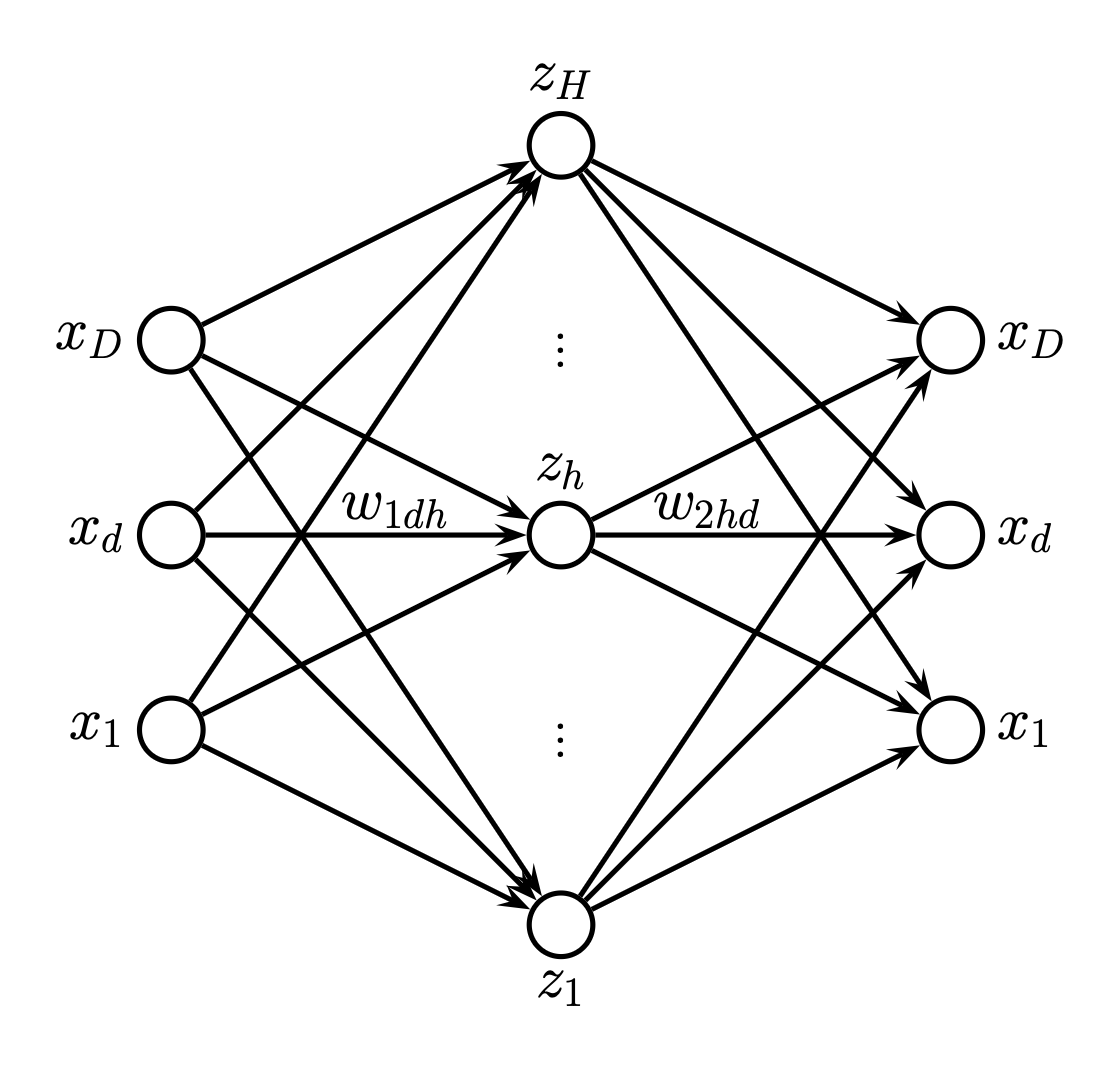
\includegraphics[width=0.4\linewidth]{images/autoencoderdemo.png}
  \caption{An autoencoder with one hidden layer MLP}
\end{figure}
\noindent The hidden units in the middle is a low-dimensional bottleneck between the input and its reconstruction.

If the hidden layer is wide enough, the model may learn the identity function. Thus, a narrow bottleneck layer with $L \ll D$ can be used, called \textbf{undercomplete representation}; a wider bottleneck layer with $L \gg D$ can also be used but to impose other kind of regularization, called \textbf{overcomplete representation}.

Regularization techniques to avoid trivial memorization,
\begin{enumerate}
    \item \textbf{Bottleneck autoencoders}: This is a special case of a \textbf{linear autoencoder}, in which there is one hidden layer, the hidden units are computed using $\boldsymbol{z} = \mathbf{W}_1\boldsymbol{x}$, and the output is reconstructed using $\hat{\boldsymbol{x}} = \mathbf{W}_2\boldsymbol{z}$, where $\mathbf{W}_1$ is a $L \times D$ matrix, $\mathbf{W}_2$ is a $D \times L$ matrix, and $L < D$ (restricting model capacity). Hence $\hat{\boldsymbol{x}} = \mathbf{W}_2\mathbf{W}_1\boldsymbol{x} = \mathbf{W}\boldsymbol{x}$ is the output of the model. If we train this model to minimize the squared reconstruction error, $\mathcal{L}(\mathbf{W}) = \sum_{n=1}^N \|\boldsymbol{x}_n - \mathbf{W}\boldsymbol{x}_n\|_2^2$, literature shows that $\hat{\mathbf{W}}$ is an orthogonal projection onto the first $L$ eigenvectors of the empirical covariance matrix of the data, equivalent to PCA. If non-linearities are introduced, such as replacing MLP with CNN, the model is strictly more powerful than PCA without significantly changes the model size and training time.
    \begin{figure}[H]
    \centering
    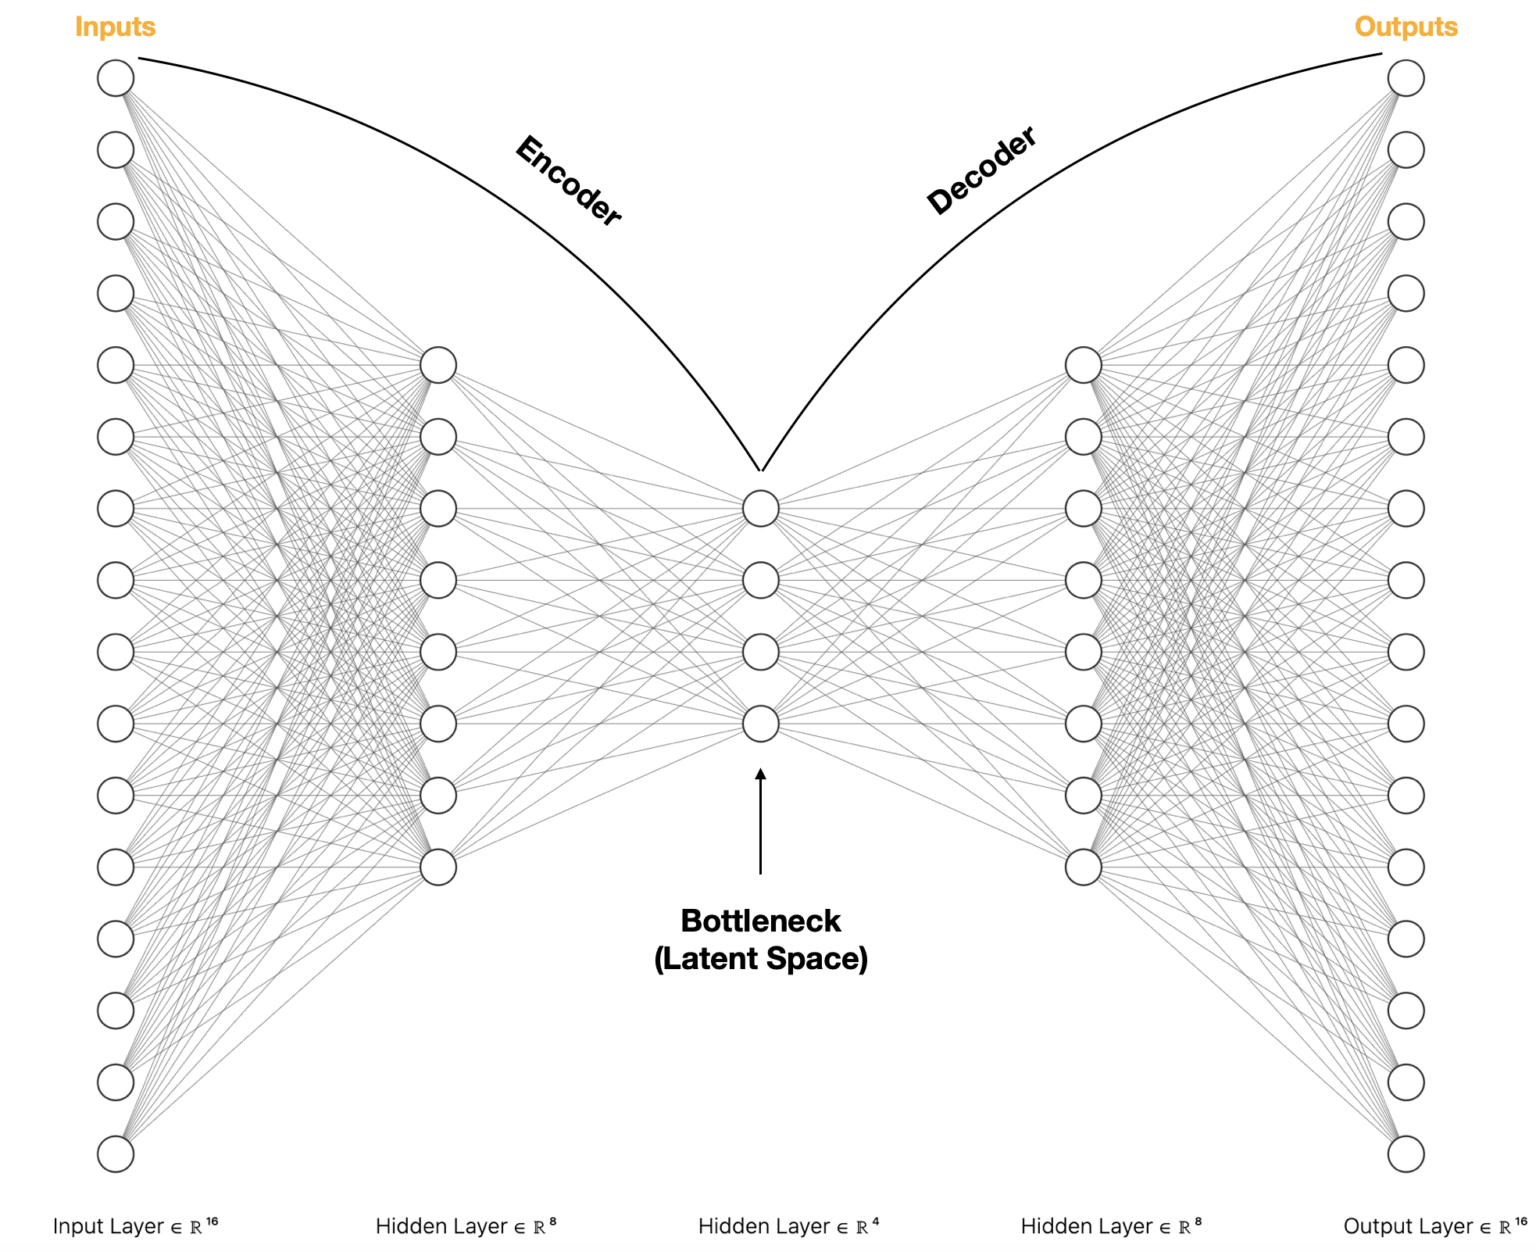
\includegraphics[width=0.5\linewidth]{images/bottleneckAE.png}
    \caption{Schematic illustration of an undercomplete autoencoder.}
    \end{figure}
    \item \textbf{Denoising autoencoders}: Adding noises such as Gaussian noise to the input, the model is able to recover details that are missing in the input, since it has seen similar images before, and can store this information in the parameters of the model. Suppose we train a DAE using Gaussian corruption and squared error reconstruction, i.e., we use $p_c(\tilde{\boldsymbol{x}} \mid \boldsymbol{x}) = \mathcal{N}(\tilde{\boldsymbol{x}} \mid \boldsymbol{x}, \sigma^2 \mathbf{I})$ and $\ell(\boldsymbol{x}, r(\tilde{\boldsymbol{x}})) = \|\boldsymbol{r(\tilde{\boldsymbol{x}}) - \boldsymbol{x}}\|_2^2$ for sample $\boldsymbol{x}$. DAE can learn a vector field, corresponding to the gradient of the log data density $\boldsymbol{e}(\boldsymbol{x}) = r(\tilde{\boldsymbol{x}}) - \boldsymbol{x} \approx \nabla_{\boldsymbol{x}} \log p(\boldsymbol{x})$. Thus points that are close to the data manifold will be projected onto it via the sampling process.
    \item \textbf{Contractive autoencoders}: Adding a penalty term to the reconstruction loss, $\lambda \left\| \frac{\partial f_e(\boldsymbol{x})}{\partial \boldsymbol{x}} \right\|_F^2 = \lambda \sum_k \|\nabla_{\boldsymbol{x}} h_k(\boldsymbol{x})\|_2^2$ (i.e. penalize the Frobenius norm of the encoder's Jacobian), forcing the encoding to be insensitive to small input perturbations.
    \item \textbf{Sparse autoencoders}: Adding a penalty term to the reconstruction loss, $\lambda \left\| \boldsymbol{z} \right\|_1$, forcing some embeddings to be small/zero. Thus, even under the overcomplete representation ($L > D$), it restricts how much of the model capacity gets used at any one time, which can actually give a richer, more interpretable representation
\end{enumerate}

In summary, the workflow of a deterministic autoencoder is as follows

\textbf{Setup}\begin{itemize}
    \item Input $\boldsymbol{x} \in \mathbb{R}^D$ (high-dim), latent $\boldsymbol{z} \in \mathbb{R}^K$ with $K \ll D$
    \item Encoder $f_e(\boldsymbol{x};\boldsymbol{\phi}): \mathbb{R}^D \to \mathbb{R}^K$
    \item Decoder $f_d(\boldsymbol{z};\boldsymbol{\theta}): \mathbb{R}^K \to \mathbb{R}^D$
\end{itemize}

\textbf{Training steps}
\begin{enumerate}
    \item Sample a minibatch $\{\boldsymbol{x}_i\}$ from the dataset
    \item Forward pass: $\boldsymbol{z}_i = f_e(\boldsymbol{x}_i;\boldsymbol{\phi})$ (deterministic, single vector --- no sampling)
    \item Reconstruct: $\hat{\boldsymbol{x}}_i = f_d(\boldsymbol{z}_i;\boldsymbol{\theta})$
    \item Compute loss:
    \[
        \mathcal{L} = \frac{1}{N}\sum_{i} \|\boldsymbol{x}_i - \hat{\boldsymbol{x}}_i\|^2
    \]
    (or cross-entropy, depending on data type)
    \item Backprop $\nabla_{\boldsymbol{\theta}} \mathcal{L}, \nabla_{\boldsymbol{\phi}} \mathcal{L}$, and update $\boldsymbol{\theta}, \boldsymbol{\phi}$ with an optimizer (Adam, SGD, etc.)
    \item Repeat over epochs until convergence
\end{enumerate}

\textbf{Inference}
Taking a new/held-out point $\boldsymbol{x}$, passing it through the encoder $\boldsymbol{z} = f_e(\boldsymbol{x};\boldsymbol{\phi})$, where $\boldsymbol{z} \in \mathbb{R}^K$ is the reduced-dimension representation. Passing through the decoder if reconstruction is needed.

\subsection{Variational autoencoders (VAE)}
\begin{table}[H]
\centering
\renewcommand{\arraystretch}{1.4}
\begin{tabular}{|p{2.6cm}|p{8cm}|p{3cm}|}
\hline
& \textbf{Deterministic} & \textbf{Probabilistic} \\
\hline
\textit{Linear} &
PCA &
PPCA, FA \\
\hline
\textit{Nonlinear} &
Bottleneck/Denoising/Contractive/Sparse AE &
VAE \\
\hline
\end{tabular}
\caption{Comparison of dimensionality reduction algorithms.}
\end{table}

VAE can be thought of as a probabilistic version of the deterministic autoencoder. Thus, as a generative model, it can generate new samples instead of just computing embeddings of input vectors.

Also, VAE is the non-linear extension of the factor analysis generative model. Replacing $p(\boldsymbol{x} \mid \boldsymbol{z}) = \mathcal{N}(\boldsymbol{x} \mid \mathbf{W}\boldsymbol{z}, \sigma^2\mathbf{I})$ with 
\[
p_{\boldsymbol{\theta}}(\boldsymbol{x} \mid \boldsymbol{z}) = \mathcal{N}(\boldsymbol{x} \mid f_d(\boldsymbol{z}; \boldsymbol{\theta}), \sigma^2\mathbf{I})
\]
where $f_d$ is a non-linear decoder with parameter $\boldsymbol{\theta}$.

Since the posterior $p(\boldsymbol{z} \mid \boldsymbol{x})$ is intractable, so another model $q(\boldsymbol{z} \mid \boldsymbol{x})$ is created to approximate the posterior, called recognition network or inference network. If the posterior is assumed to be Gaussian, with diagonal covariance, then,
\[
q_{\boldsymbol{\phi}}(\boldsymbol{z} \mid \boldsymbol{x}) = \mathcal{N}(\boldsymbol{z} \mid f_{e,\mu}(\boldsymbol{x}; \boldsymbol{\phi}), \text{diag}(f_{e,\sigma}(\boldsymbol{x}; \boldsymbol{\phi})))
\]
where $f_{e, \mu /\sigma}$ is the encoder for mean and variance respectively with parameter $\boldsymbol{\phi}$. This idea of training an inference network to invert a generative network, rather than running an optimization algorithm to infer the latent code, is called amortized inference.

\begin{figure}[H]
  \centering
  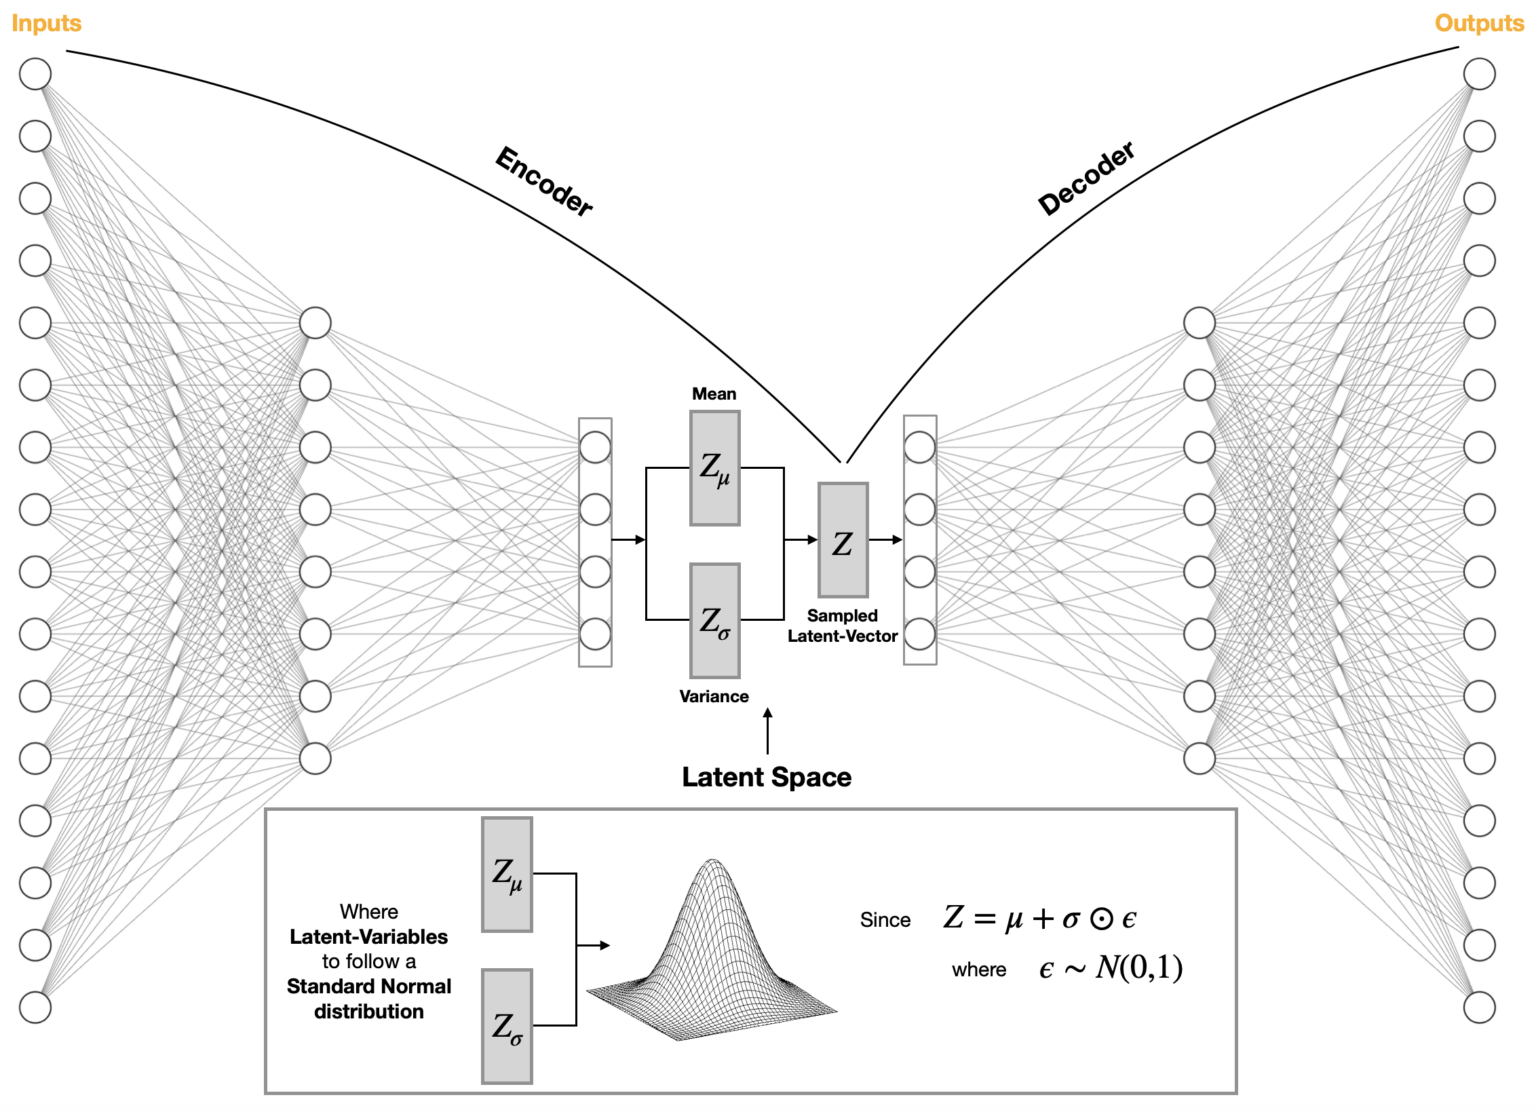
\includegraphics[width=0.5\linewidth]{images/VAE.png}
  \caption{Schematic illustration of a VAE.}
\end{figure}

\subsection*{Training VAEs}
The computation of exact $p_{\boldsymbol{\theta}}(\boldsymbol{x}) = \int p_{\boldsymbol{\theta}}(\boldsymbol{x}, \boldsymbol{z}) d\boldsymbol z = \int p_{\boldsymbol{\theta}}(\boldsymbol{x} \mid \boldsymbol{z}) p(\boldsymbol{z}) d\boldsymbol{z}$ for MLE training is in possible because the porterior in a nonlinear FA model is intractable. However, by making use of $q(\boldsymbol{z} \mid \boldsymbol{x})$, ELBO can be computed. For a single example $\boldsymbol{x}$, the ELBO as the objective function is,
\[
\begin{aligned}
\text{L}(\boldsymbol{\theta}, \boldsymbol{\phi} | \boldsymbol{x}) &= \mathbb{E}_{q_{\boldsymbol{\phi}}(\boldsymbol{z}|\boldsymbol{x})} \left[ \log p_{\boldsymbol{\theta}}(\boldsymbol{x}, \boldsymbol{z}) - \log q_{\boldsymbol{\phi}}(\boldsymbol{z}|\boldsymbol{x}) \right] \\
&= \mathbb{E}_{q(\boldsymbol{z}|\boldsymbol{x}, \boldsymbol{\phi})} \left[ \log p(\boldsymbol{x}|\boldsymbol{z}, \boldsymbol{\theta}) \right] - D_{KL} \left( q(\boldsymbol{z}|\boldsymbol{x}, \boldsymbol{\phi}) \, \| \, p(\boldsymbol{z}) \right)
\end{aligned}
\]
where $q_{\boldsymbol{\phi}}(\boldsymbol{z}|\boldsymbol{x}) = q(\boldsymbol{z}|\boldsymbol{x}, \boldsymbol{\phi})$ are different notation conventions. This can be interpreted as the expected log-likelihood plus a regularizer which penalizes the posterior from deviating too much from the prior.

ELBO is a lower bound of the evidence as shown by the Jensen's inquality,
\[
\begin{aligned}
\text{L}(\boldsymbol{\theta}, \boldsymbol{\phi} | \boldsymbol{x}) &= \int q_{\boldsymbol{\phi}}(\boldsymbol{z}|\boldsymbol{x}) \log \frac{p_{\boldsymbol{\theta}}(\boldsymbol{x}, \boldsymbol{z})}{q_{\boldsymbol{\phi}}(\boldsymbol{z}|\boldsymbol{x})} d\boldsymbol{z} \\
&\leq \log \int q_{\boldsymbol{\phi}}(\boldsymbol{z}|\boldsymbol{x}) \frac{p_{\boldsymbol{\theta}}(\boldsymbol{x}, \boldsymbol{z})}{q_{\boldsymbol{\phi}}(\boldsymbol{z}|\boldsymbol{x})} d\boldsymbol{z} = \log p_{\boldsymbol{\theta}}(\boldsymbol{x})
\end{aligned}
\]
Thus, the optimization task for training VAE is 
\[
\boldsymbol{\theta}^*, \boldsymbol{\phi}^* = \arg\max_{\boldsymbol{\theta}, \boldsymbol{\phi}} \, \sum_i \mathcal{L}(\boldsymbol{\theta}, \boldsymbol{\phi} \mid \boldsymbol{x})
\]

A trick in computing ELBO is \textbf{reparameterization}. Since $q_{\boldsymbol{\phi}}(\boldsymbol{z}|\boldsymbol{x})$ is Gaussian, then 
\[
\boldsymbol{z} = f_{e,\mu}(\boldsymbol{x}; \boldsymbol{\phi}) + f_{e,\sigma}(\boldsymbol{x}; \boldsymbol{\phi}) \odot \boldsymbol{\epsilon}
\]
where $\boldsymbol{\epsilon} \sim \mathcal{N}(\boldsymbol{0}, \boldsymbol{I})$ and $\odot$ denotes element-wise multiplication. Hence,
\[
\text{L}(\boldsymbol{\theta}, \boldsymbol{\phi} | \boldsymbol{x}) = \mathbb{E}_{\boldsymbol{\epsilon} \sim \mathcal{N}(\boldsymbol{0}, \mathbf{I})} \left[ \log p{\boldsymbol{\theta}}(\boldsymbol{x} | \boldsymbol{z} = \mu_{\boldsymbol{\phi}}(\boldsymbol{x}) + \sigma_{\boldsymbol{\phi}}(\boldsymbol{x}) \odot \boldsymbol{\epsilon}) \right] - D_{KL} \left( q_{\boldsymbol{\phi}}(\boldsymbol{z}|\boldsymbol{x}) \mid p(\boldsymbol{z}) \right)
\]
The expectation is now over a fixed distribution $\boldsymbol{\epsilon} \sim \mathcal{N}(\boldsymbol{0}, \boldsymbol{I})$. Before reparameterization, every gradient step would change $q_{\boldsymbol{\phi}}(\boldsymbol{z}|\boldsymbol{x})$ itself (the ground samples are taking from shifts). After reparameterization, always sampling from the same fixed source of randomness $\boldsymbol{\epsilon}$, and all the parameter($\boldsymbol{\phi}$)-dependence has been moved into a deterministic, differentiable path inside the expectation (i.e. once $\boldsymbol{\epsilon}$ is sampled, only a deterministic and differentiable neural network $f_{e, \mu / \sigma}$ is left). Therefore, the backpropagation for training can be used as usual.

The first term in the ELBO can be approximated by sampling $\boldsymbol{\epsilon}$, scaling it by the output of the inference network to get $\boldsymbol{z}$, and then evaluating $\log p(\boldsymbol{x}|\boldsymbol{z})$ using the decoder network $f_d$.

The second term in the ELBO is the KL of two Gaussians, which has a closed form expression. With $p(\boldsymbol{z}) = \mathcal{N}(\boldsymbol{z}|\boldsymbol{0}, \mathbf{I})$ and $q_{\boldsymbol{\phi}}(\boldsymbol{z} \mid \boldsymbol{x}) = \mathcal{N}(\boldsymbol{z}|\boldsymbol{\mu}, \text{diag}(\boldsymbol{\sigma}))$,
\[
D_{KL}\left(q \| p\right) = \sum_{k=1}^{K} \left[ \log\left(\frac{1}{\sigma_k}\right) + \frac{\sigma_k^2 + (\mu_k - 0)^2}{2 \cdot 1} - \frac{1}{2} \right] = -\frac{1}{2} \sum_{k=1}^{K} \left[ \log \sigma_k^2 - \sigma_k^2 - \mu_k^2 + 1 \right]
\]

\begin{figure}[H]
  \centering
  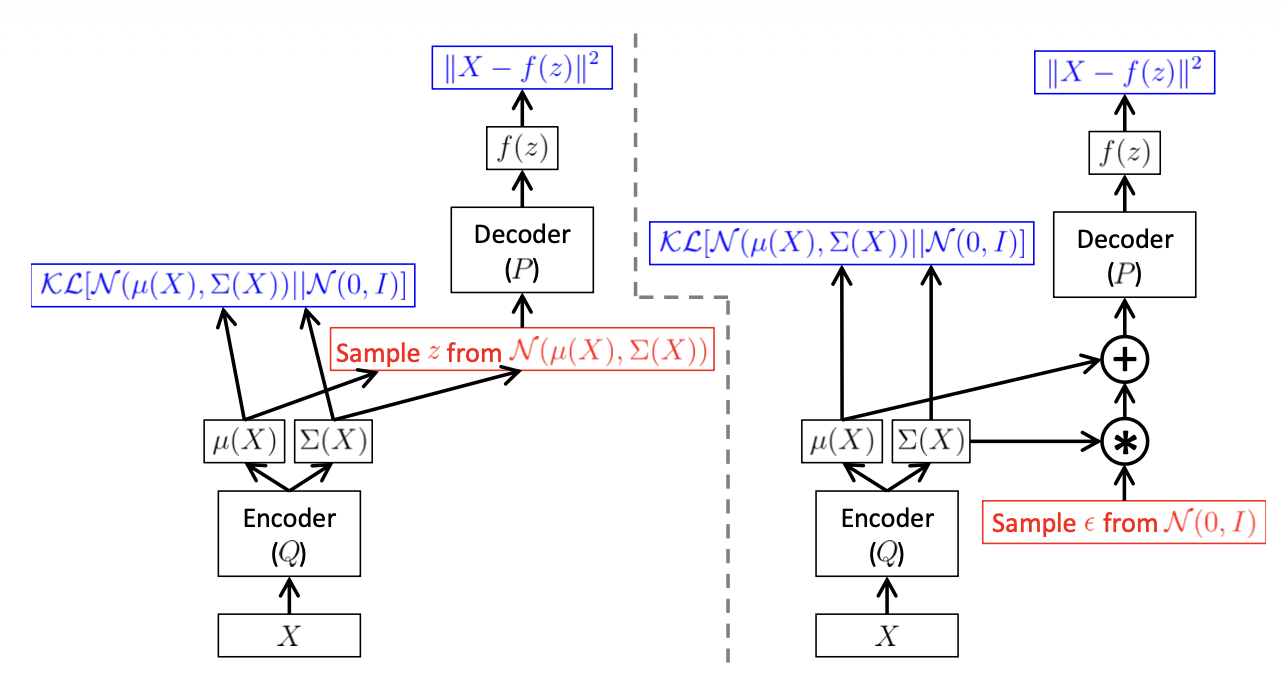
\includegraphics[width=0.5\linewidth]{images/reparameterization.png}
  \caption{Computation graphs for VAEs. Computation graph for VAEs, where $p(\boldsymbol{z}) = \mathcal{N}(\boldsymbol{z}|\boldsymbol{0}, \mathbf{I})$, $p(\boldsymbol{x}|\boldsymbol{z}, \boldsymbol{\theta}) = \mathcal{N}(\boldsymbol{x}|f(\boldsymbol{z}), \sigma^2 \mathbf{I})$, and $q(\boldsymbol{z}|\boldsymbol{x}, \boldsymbol{\phi}) = \mathcal{N}(\boldsymbol{z}|\mu(\boldsymbol{x}), \Sigma(\boldsymbol{x}))$. Red boxes show sampling operations which are not differentiable. Blue boxes show loss layers (we assume Gaussian likelihoods and priors). (Left) Without the reparameterization trick. (Right) With the reparameterization trick. Gradients can flow from the output loss, back through the decoder and into the encoder.}
\end{figure}

In summary, 

\textbf{Setup}
\begin{itemize}
    \item $\boldsymbol{x} \in \mathbb{R}^D$, $\boldsymbol{z} \in \mathbb{R}^K$
    \item Encoder outputs distribution params: $\mu_{\boldsymbol{\phi}}(\boldsymbol{x}), \sigma_{\boldsymbol{\phi}}(\boldsymbol{x}) \in \mathbb{R}^K$
    \item Decoder $f_d(\boldsymbol{z};\boldsymbol{\theta})$ outputs likelihood params for $p_{\boldsymbol{\theta}}(\boldsymbol{x}|\boldsymbol{z})$
    \item Fixed prior $p(\boldsymbol{z}) = \mathcal{N}(0,I)$
\end{itemize}

\textbf{Training steps}
\begin{enumerate}
    \item Sample a minibatch $\{\boldsymbol{x}_i\}$, then forward pass through encoder: $(\mu_{\boldsymbol{\phi}}(\boldsymbol{x}_i), \sigma_{\boldsymbol{\phi}}(\boldsymbol{x}_i)) = f_e(\boldsymbol{x}_i;\boldsymbol{\phi})$
    \item Reparameterize: $\boldsymbol{z}_i = \mu_{\boldsymbol{\phi}}(\boldsymbol{x}_i) + \sigma_{\boldsymbol{\phi}}(\boldsymbol{x}_i)\odot \boldsymbol{\epsilon}$ (deterministic given $\boldsymbol{\epsilon}$, differentiable w.r.t.\ $\boldsymbol{\phi}$) with a sample from $\boldsymbol{\epsilon} \sim \mathcal{N}(0,I)$
    \item Decode: pass $\boldsymbol{z}_i$ through decoder to get $p_{\boldsymbol{\theta}}(\boldsymbol{x}|\boldsymbol{z}_i)$'s parameters, which can be used for ELBO first term calculation.
    \item Compute ELBO:
    \[
        \mathcal{L}(\boldsymbol{\theta},\boldsymbol{\phi} \mid \boldsymbol{x}_i) = \log p_{\boldsymbol{\theta}}(\boldsymbol{x}_i \mid \boldsymbol{z}_i) - D_{KL}\big(q_{\boldsymbol{\phi}}(\boldsymbol{z} \mid \boldsymbol{x}_i)\,\|\,p(\boldsymbol{z})\big)
    \]
    \item Minimize $-\dfrac{1}{N}\sum_{i} \mathcal{L}(\boldsymbol{\theta},\boldsymbol{\phi} \mid \boldsymbol{x}_i)$ via backprop --- gradients flow through the reparameterized $\boldsymbol{z}_i$ into both $\boldsymbol{\phi}$ and $\boldsymbol{\theta}$, and update $\boldsymbol{\theta}, \boldsymbol{\phi}$ with an optimizer
    \item Repeat over epochs
\end{enumerate}

\textbf{Inference}
Here there is a choice, since the encoder gives a \emph{distribution}, not a point:
\begin{itemize}
    \item Option A: use the mean only, $\boldsymbol{z} = \mu_{\boldsymbol{\phi}}(\boldsymbol{x})$, as the reduced representation --- deterministic, ignores $\sigma_{\boldsymbol{\phi}}(\boldsymbol{x})$ entirely. This is typical when a fixed embedding is needed (e.g.\ for downstream clustering/visualization).
    \item Option B: sample $\boldsymbol{z} \sim q_{\boldsymbol{\phi}}(\boldsymbol{z}\mid \boldsymbol{x}) = \mathcal{N}(\mu_{\boldsymbol{\phi}}(\boldsymbol{x}), \sigma_{\boldsymbol{\phi}}(\boldsymbol{x})^2)$ each time --- introduces stochasticity into the reduced representation.
\end{itemize}
Key property: because of the KL regularization during training, the resulting $\boldsymbol{z}$-space (using $\mu_{\boldsymbol{\phi}}(\boldsymbol{x})$) tends to be smoother and better organized around the origin than a plain AE's latent space, at some cost to reconstruction fidelity (since the KL term competes with the reconstruction term).

\end{document}
